% Options for packages loaded elsewhere
\PassOptionsToPackage{unicode}{hyperref}
\PassOptionsToPackage{hyphens}{url}
\PassOptionsToPackage{dvipsnames,svgnames,x11names}{xcolor}
%
\documentclass[
  letterpaper,
]{krantz}

\usepackage{amsmath,amssymb}
\usepackage{lmodern}
\usepackage{iftex}
\ifPDFTeX
  \usepackage[T1]{fontenc}
  \usepackage[utf8]{inputenc}
  \usepackage{textcomp} % provide euro and other symbols
\else % if luatex or xetex
  \usepackage{unicode-math}
  \defaultfontfeatures{Scale=MatchLowercase}
  \defaultfontfeatures[\rmfamily]{Ligatures=TeX,Scale=1}
\fi
% Use upquote if available, for straight quotes in verbatim environments
\IfFileExists{upquote.sty}{\usepackage{upquote}}{}
\IfFileExists{microtype.sty}{% use microtype if available
  \usepackage[]{microtype}
  \UseMicrotypeSet[protrusion]{basicmath} % disable protrusion for tt fonts
}{}
\makeatletter
\@ifundefined{KOMAClassName}{% if non-KOMA class
  \IfFileExists{parskip.sty}{%
    \usepackage{parskip}
  }{% else
    \setlength{\parindent}{0pt}
    \setlength{\parskip}{6pt plus 2pt minus 1pt}}
}{% if KOMA class
  \KOMAoptions{parskip=half}}
\makeatother
\usepackage{xcolor}
\usepackage[normalem]{ulem}
\setlength{\emergencystretch}{3em} % prevent overfull lines
\setcounter{secnumdepth}{5}
% Make \paragraph and \subparagraph free-standing
\ifx\paragraph\undefined\else
  \let\oldparagraph\paragraph
  \renewcommand{\paragraph}[1]{\oldparagraph{#1}\mbox{}}
\fi
\ifx\subparagraph\undefined\else
  \let\oldsubparagraph\subparagraph
  \renewcommand{\subparagraph}[1]{\oldsubparagraph{#1}\mbox{}}
\fi

\usepackage{color}
\usepackage{fancyvrb}
\newcommand{\VerbBar}{|}
\newcommand{\VERB}{\Verb[commandchars=\\\{\}]}
\DefineVerbatimEnvironment{Highlighting}{Verbatim}{commandchars=\\\{\}}
% Add ',fontsize=\small' for more characters per line
\usepackage{framed}
\definecolor{shadecolor}{RGB}{241,243,245}
\newenvironment{Shaded}{\begin{snugshade}}{\end{snugshade}}
\newcommand{\AlertTok}[1]{\textcolor[rgb]{0.68,0.00,0.00}{#1}}
\newcommand{\AnnotationTok}[1]{\textcolor[rgb]{0.37,0.37,0.37}{#1}}
\newcommand{\AttributeTok}[1]{\textcolor[rgb]{0.40,0.45,0.13}{#1}}
\newcommand{\BaseNTok}[1]{\textcolor[rgb]{0.68,0.00,0.00}{#1}}
\newcommand{\BuiltInTok}[1]{\textcolor[rgb]{0.00,0.23,0.31}{#1}}
\newcommand{\CharTok}[1]{\textcolor[rgb]{0.13,0.47,0.30}{#1}}
\newcommand{\CommentTok}[1]{\textcolor[rgb]{0.37,0.37,0.37}{#1}}
\newcommand{\CommentVarTok}[1]{\textcolor[rgb]{0.37,0.37,0.37}{\textit{#1}}}
\newcommand{\ConstantTok}[1]{\textcolor[rgb]{0.56,0.35,0.01}{#1}}
\newcommand{\ControlFlowTok}[1]{\textcolor[rgb]{0.00,0.23,0.31}{#1}}
\newcommand{\DataTypeTok}[1]{\textcolor[rgb]{0.68,0.00,0.00}{#1}}
\newcommand{\DecValTok}[1]{\textcolor[rgb]{0.68,0.00,0.00}{#1}}
\newcommand{\DocumentationTok}[1]{\textcolor[rgb]{0.37,0.37,0.37}{\textit{#1}}}
\newcommand{\ErrorTok}[1]{\textcolor[rgb]{0.68,0.00,0.00}{#1}}
\newcommand{\ExtensionTok}[1]{\textcolor[rgb]{0.00,0.23,0.31}{#1}}
\newcommand{\FloatTok}[1]{\textcolor[rgb]{0.68,0.00,0.00}{#1}}
\newcommand{\FunctionTok}[1]{\textcolor[rgb]{0.28,0.35,0.67}{#1}}
\newcommand{\ImportTok}[1]{\textcolor[rgb]{0.00,0.46,0.62}{#1}}
\newcommand{\InformationTok}[1]{\textcolor[rgb]{0.37,0.37,0.37}{#1}}
\newcommand{\KeywordTok}[1]{\textcolor[rgb]{0.00,0.23,0.31}{#1}}
\newcommand{\NormalTok}[1]{\textcolor[rgb]{0.00,0.23,0.31}{#1}}
\newcommand{\OperatorTok}[1]{\textcolor[rgb]{0.37,0.37,0.37}{#1}}
\newcommand{\OtherTok}[1]{\textcolor[rgb]{0.00,0.23,0.31}{#1}}
\newcommand{\PreprocessorTok}[1]{\textcolor[rgb]{0.68,0.00,0.00}{#1}}
\newcommand{\RegionMarkerTok}[1]{\textcolor[rgb]{0.00,0.23,0.31}{#1}}
\newcommand{\SpecialCharTok}[1]{\textcolor[rgb]{0.37,0.37,0.37}{#1}}
\newcommand{\SpecialStringTok}[1]{\textcolor[rgb]{0.13,0.47,0.30}{#1}}
\newcommand{\StringTok}[1]{\textcolor[rgb]{0.13,0.47,0.30}{#1}}
\newcommand{\VariableTok}[1]{\textcolor[rgb]{0.07,0.07,0.07}{#1}}
\newcommand{\VerbatimStringTok}[1]{\textcolor[rgb]{0.13,0.47,0.30}{#1}}
\newcommand{\WarningTok}[1]{\textcolor[rgb]{0.37,0.37,0.37}{\textit{#1}}}

\providecommand{\tightlist}{%
  \setlength{\itemsep}{0pt}\setlength{\parskip}{0pt}}\usepackage{longtable,booktabs,array}
\usepackage{calc} % for calculating minipage widths
% Correct order of tables after \paragraph or \subparagraph
\usepackage{etoolbox}
\makeatletter
\patchcmd\longtable{\par}{\if@noskipsec\mbox{}\fi\par}{}{}
\makeatother
% Allow footnotes in longtable head/foot
\IfFileExists{footnotehyper.sty}{\usepackage{footnotehyper}}{\usepackage{footnote}}
\makesavenoteenv{longtable}
\usepackage{graphicx}
\makeatletter
\def\maxwidth{\ifdim\Gin@nat@width>\linewidth\linewidth\else\Gin@nat@width\fi}
\def\maxheight{\ifdim\Gin@nat@height>\textheight\textheight\else\Gin@nat@height\fi}
\makeatother
% Scale images if necessary, so that they will not overflow the page
% margins by default, and it is still possible to overwrite the defaults
% using explicit options in \includegraphics[width, height, ...]{}
\setkeys{Gin}{width=\maxwidth,height=\maxheight,keepaspectratio}
% Set default figure placement to htbp
\makeatletter
\def\fps@figure{htbp}
\makeatother
\newlength{\cslhangindent}
\setlength{\cslhangindent}{1.5em}
\newlength{\csllabelwidth}
\setlength{\csllabelwidth}{3em}
\newlength{\cslentryspacingunit} % times entry-spacing
\setlength{\cslentryspacingunit}{\parskip}
\newenvironment{CSLReferences}[2] % #1 hanging-ident, #2 entry spacing
 {% don't indent paragraphs
  \setlength{\parindent}{0pt}
  % turn on hanging indent if param 1 is 1
  \ifodd #1
  \let\oldpar\par
  \def\par{\hangindent=\cslhangindent\oldpar}
  \fi
  % set entry spacing
  \setlength{\parskip}{#2\cslentryspacingunit}
 }%
 {}
\usepackage{calc}
\newcommand{\CSLBlock}[1]{#1\hfill\break}
\newcommand{\CSLLeftMargin}[1]{\parbox[t]{\csllabelwidth}{#1}}
\newcommand{\CSLRightInline}[1]{\parbox[t]{\linewidth - \csllabelwidth}{#1}\break}
\newcommand{\CSLIndent}[1]{\hspace{\cslhangindent}#1}

\usepackage{booktabs}
\usepackage{longtable}
\usepackage{array}
\usepackage{multirow}
\usepackage{wrapfig}
\usepackage{float}
\usepackage{colortbl}
\usepackage{pdflscape}
\usepackage{tabu}
\usepackage{threeparttable}
\usepackage{threeparttablex}
\usepackage[normalem]{ulem}
\usepackage{makecell}
\usepackage{xcolor}
\makeatletter
\@ifpackageloaded{tcolorbox}{}{\usepackage[many]{tcolorbox}}
\@ifpackageloaded{fontawesome5}{}{\usepackage{fontawesome5}}
\definecolor{quarto-callout-color}{HTML}{909090}
\definecolor{quarto-callout-note-color}{HTML}{0758E5}
\definecolor{quarto-callout-important-color}{HTML}{CC1914}
\definecolor{quarto-callout-warning-color}{HTML}{EB9113}
\definecolor{quarto-callout-tip-color}{HTML}{00A047}
\definecolor{quarto-callout-caution-color}{HTML}{FC5300}
\definecolor{quarto-callout-color-frame}{HTML}{acacac}
\definecolor{quarto-callout-note-color-frame}{HTML}{4582ec}
\definecolor{quarto-callout-important-color-frame}{HTML}{d9534f}
\definecolor{quarto-callout-warning-color-frame}{HTML}{f0ad4e}
\definecolor{quarto-callout-tip-color-frame}{HTML}{02b875}
\definecolor{quarto-callout-caution-color-frame}{HTML}{fd7e14}
\makeatother
\makeatletter
\makeatother
\makeatletter
\@ifpackageloaded{bookmark}{}{\usepackage{bookmark}}
\makeatother
\makeatletter
\@ifpackageloaded{caption}{}{\usepackage{caption}}
\AtBeginDocument{%
\ifdefined\contentsname
  \renewcommand*\contentsname{Table of contents}
\else
  \newcommand\contentsname{Table of contents}
\fi
\ifdefined\listfigurename
  \renewcommand*\listfigurename{List of Figures}
\else
  \newcommand\listfigurename{List of Figures}
\fi
\ifdefined\listtablename
  \renewcommand*\listtablename{List of Tables}
\else
  \newcommand\listtablename{List of Tables}
\fi
\ifdefined\figurename
  \renewcommand*\figurename{Figure}
\else
  \newcommand\figurename{Figure}
\fi
\ifdefined\tablename
  \renewcommand*\tablename{Table}
\else
  \newcommand\tablename{Table}
\fi
}
\@ifpackageloaded{float}{}{\usepackage{float}}
\floatstyle{ruled}
\@ifundefined{c@chapter}{\newfloat{codelisting}{h}{lop}}{\newfloat{codelisting}{h}{lop}[chapter]}
\floatname{codelisting}{Listing}
\newcommand*\listoflistings{\listof{codelisting}{List of Listings}}
\makeatother
\makeatletter
\@ifpackageloaded{caption}{}{\usepackage{caption}}
\@ifpackageloaded{subcaption}{}{\usepackage{subcaption}}
\makeatother
\makeatletter
\@ifpackageloaded{tcolorbox}{}{\usepackage[many]{tcolorbox}}
\makeatother
\makeatletter
\@ifundefined{shadecolor}{\definecolor{shadecolor}{rgb}{.97, .97, .97}}
\makeatother
\makeatletter
\makeatother
\ifLuaTeX
  \usepackage{selnolig}  % disable illegal ligatures
\fi
\IfFileExists{bookmark.sty}{\usepackage{bookmark}}{\usepackage{hyperref}}
\IfFileExists{xurl.sty}{\usepackage{xurl}}{} % add URL line breaks if available
\urlstyle{same} % disable monospaced font for URLs
\hypersetup{
  pdftitle={An Introduction to NFL Analytics with R},
  pdfauthor={Bradley J. Congelio},
  colorlinks=true,
  linkcolor={blue},
  filecolor={Maroon},
  citecolor={Blue},
  urlcolor={Blue},
  pdfcreator={LaTeX via pandoc}}

\title{An Introduction to NFL Analytics with R}
\author{Bradley J. Congelio}
\date{}

\begin{document}
\maketitle
\ifdefined\Shaded\renewenvironment{Shaded}{\begin{tcolorbox}[frame hidden, borderline west={3pt}{0pt}{shadecolor}, enhanced, boxrule=0pt, breakable, interior hidden, sharp corners]}{\end{tcolorbox}}\fi

\renewcommand*\contentsname{Table of contents}
{
\hypersetup{linkcolor=}
\setcounter{tocdepth}{2}
\tableofcontents
}
\bookmarksetup{startatroot}

\hypertarget{introduction}{%
\chapter{Introduction}\label{introduction}}

\begin{tcolorbox}[enhanced jigsaw, breakable, leftrule=.75mm, colframe=quarto-callout-note-color-frame, toptitle=1mm, rightrule=.15mm, colbacktitle=quarto-callout-note-color!10!white, colback=white, bottomrule=.15mm, bottomtitle=1mm, titlerule=0mm, coltitle=black, opacitybacktitle=0.6, title=\textcolor{quarto-callout-note-color}{\faInfo}\hspace{0.5em}{Note}, arc=.35mm, toprule=.15mm, left=2mm, opacityback=0]
\textbf{Please note:} this book is currently under contract with
\href{https://www.routledge.com/go/crc-press}{CRC Press} and is in the
writing process. \emph{Chapters that are completed are to be considered
a rough draft}. Other chapters, while listed in the table of contents to
the left, have yet to be worked on. The finished manuscript is scheduled
for submission to CRC Press by December 31, 2022. The complete,
open-source version will be ``official'' and live at that point, with
the hard copy of the book coming in early 2023.
\end{tcolorbox}

Welcome to the online home of\\
\textbf{\emph{Introduction to NFL Analytics with R}.}

\begin{figure}

{\centering 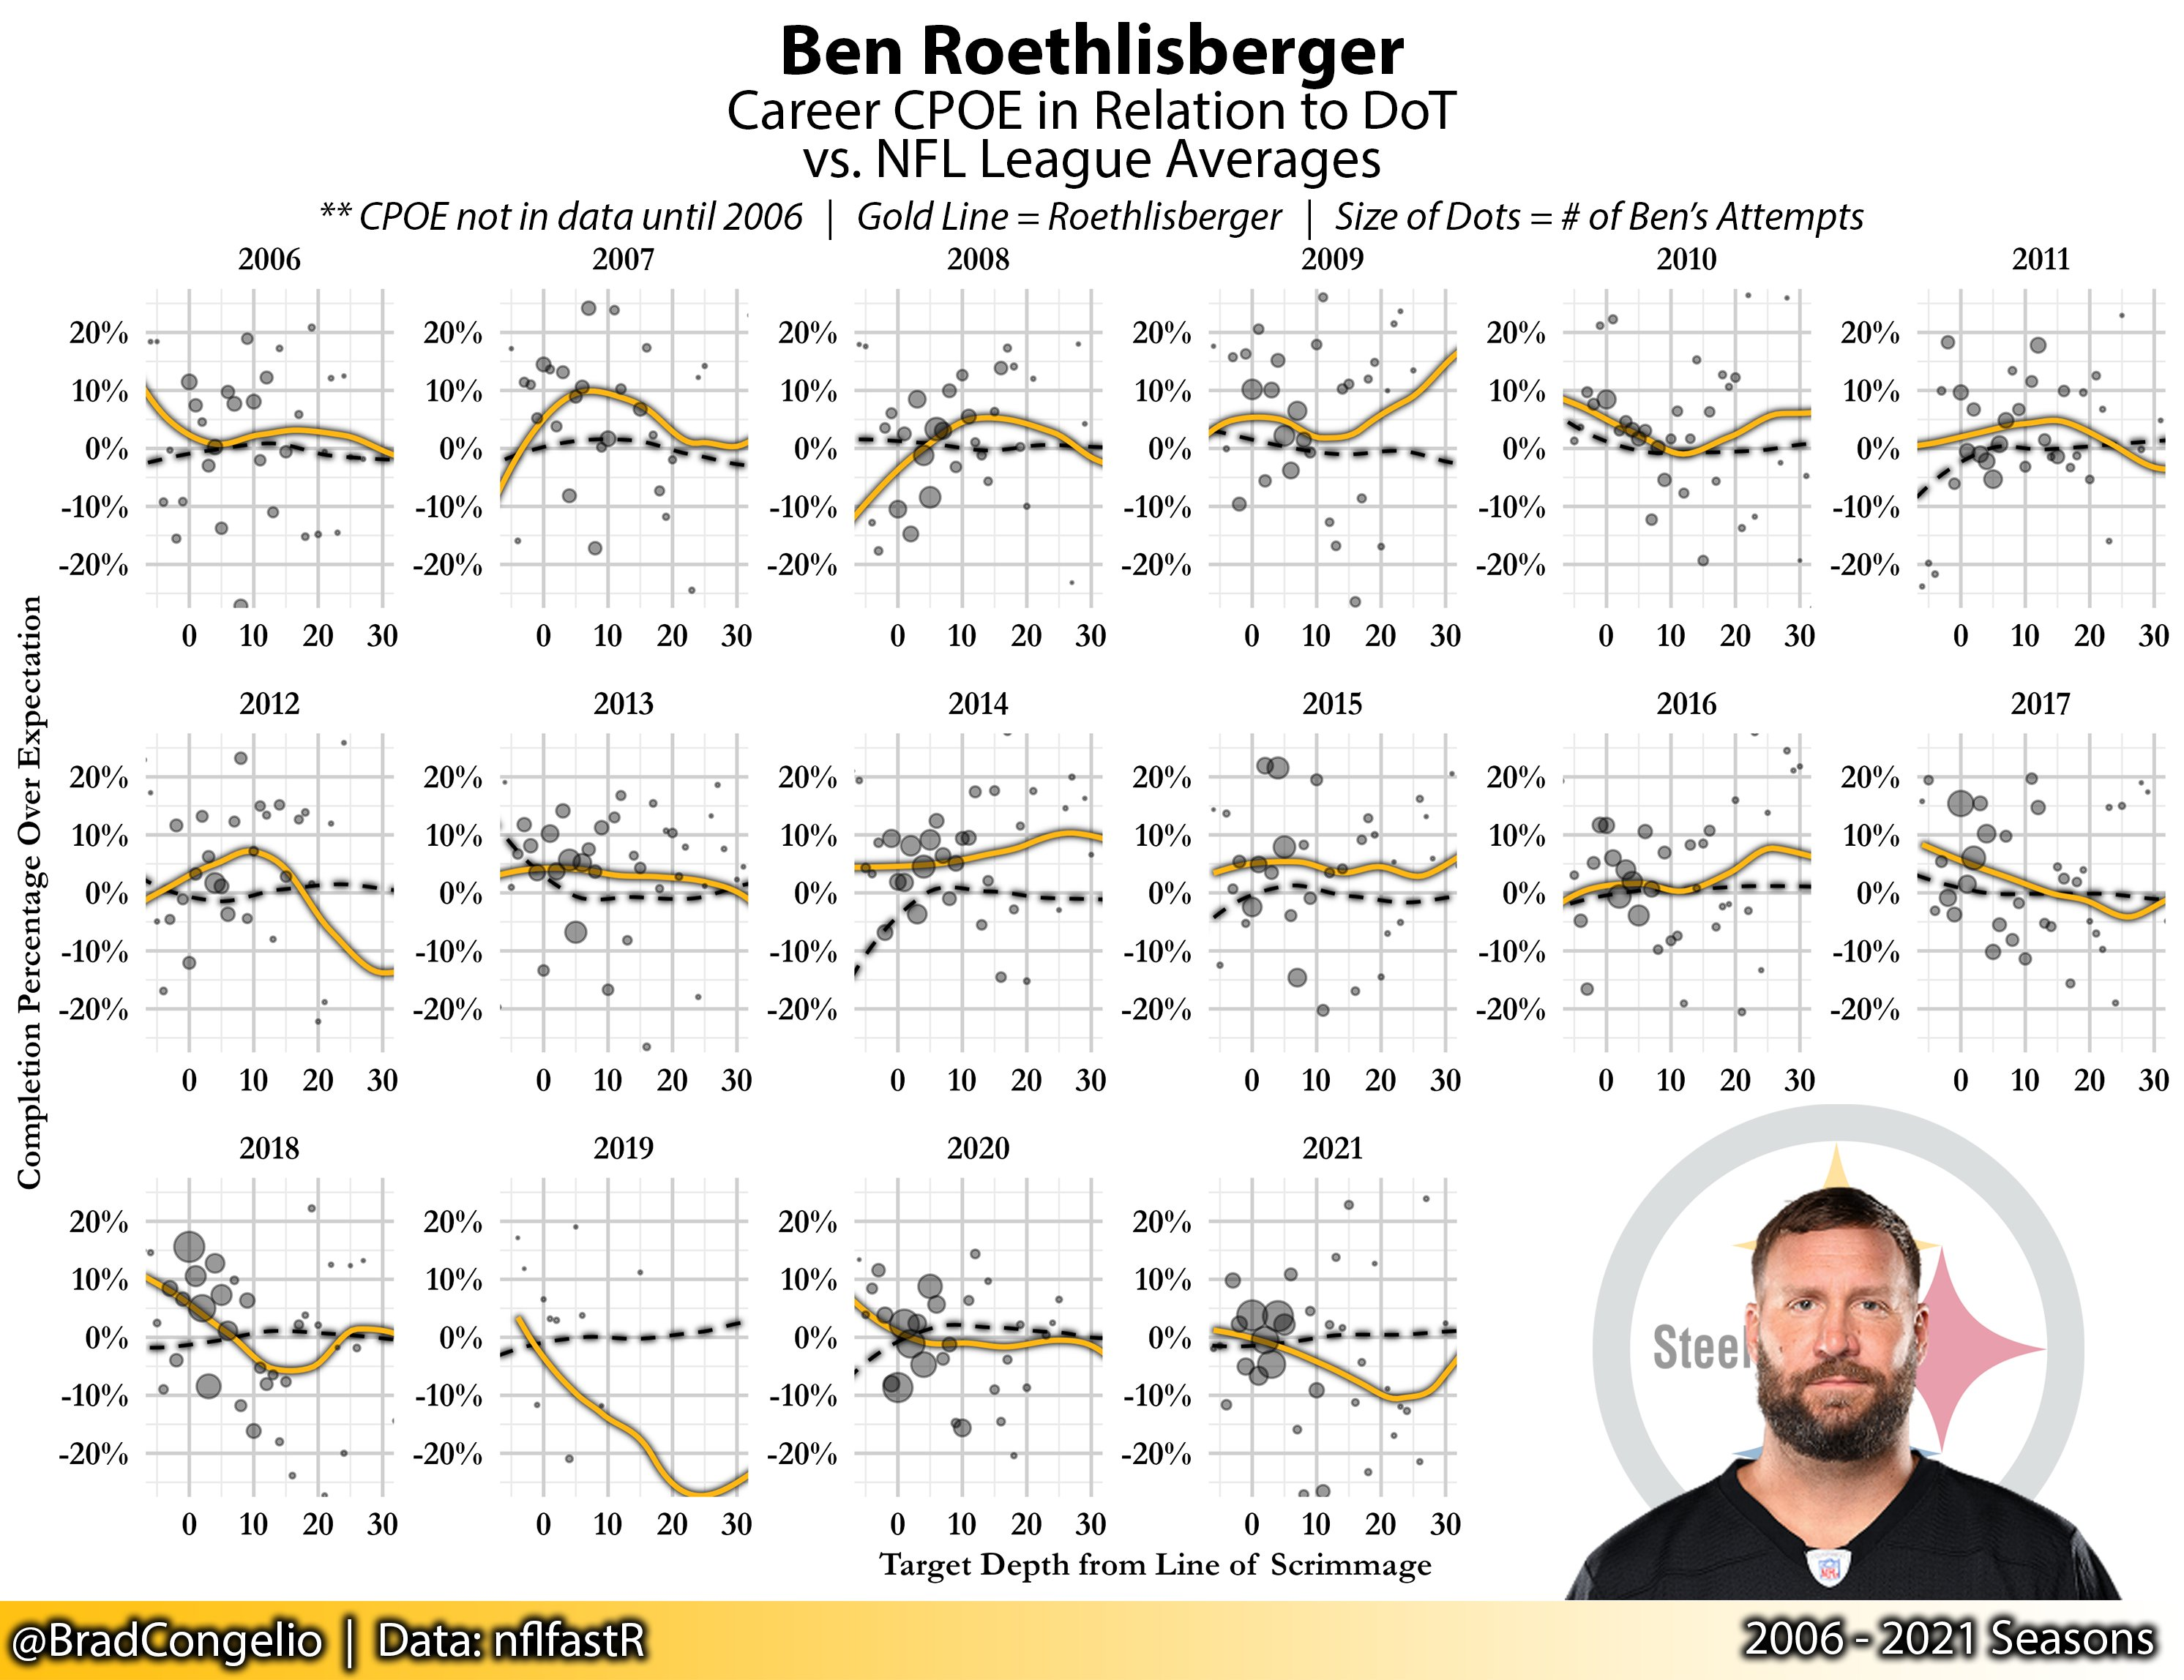
\includegraphics{./images/big-ben-intro.jpg}

}

\end{figure}

As this book is published online, it allows me to continue real-time
development of it. Because of this, make note of the following:

\begin{itemize}
\item
  \emph{Introduction to NFL Analytics with R} is currently under
  contract with CRC Press. A hard copy of the book will be avaliable for
  pre-order on Amazon and other locations in early 2023.
\item
  Please feel free to contribute to the book by filing an issue or
  making a pull request at the book's GitHub repository:
  \href{https://github.com/bcongelio/nfl-analytics-with-r-book}{\emph{Introduction
  to NFL Analytics with R} Github Repository}
\item
  The majority of the chapters conclude with exercises. In some cases,
  prepared data will be provided with a link to download the file. In
  other cases, you are expected to use the \texttt{nflverse} to collect
  the data yourself. In either case, the book's github repository for
  the exercises (link to the specific directory coming soon) will
  include the R files that contain the answers to each exercise.
\item
  Soon there will be a YouTube series to go along with the written
  version of this book. In brief, the videos will include my going over
  each chapter, step-by-step, with additional instruction and/or
  approaches.
\item
  Are you an instructor hoping to create or grow your Sport Analytics
  course? Future plans for this book include the creation of Instructor
  Materials to include an example syllabus plus structured lesson plans,
  exercises, assignments, quizzes, and exams. As well, templates for
  lectures will be included in PowerPoint form so you may edit to fit
  your specific needs.
\end{itemize}

On April 27, 2020, Ben Baldwin hit send on a Tweet that announced the
birth of \texttt{nflfastR}, an R package designed to scrape NFL
play-by-play data, allowing the end-user to access it at speeds quicker
than similar predecessors (hence the name).

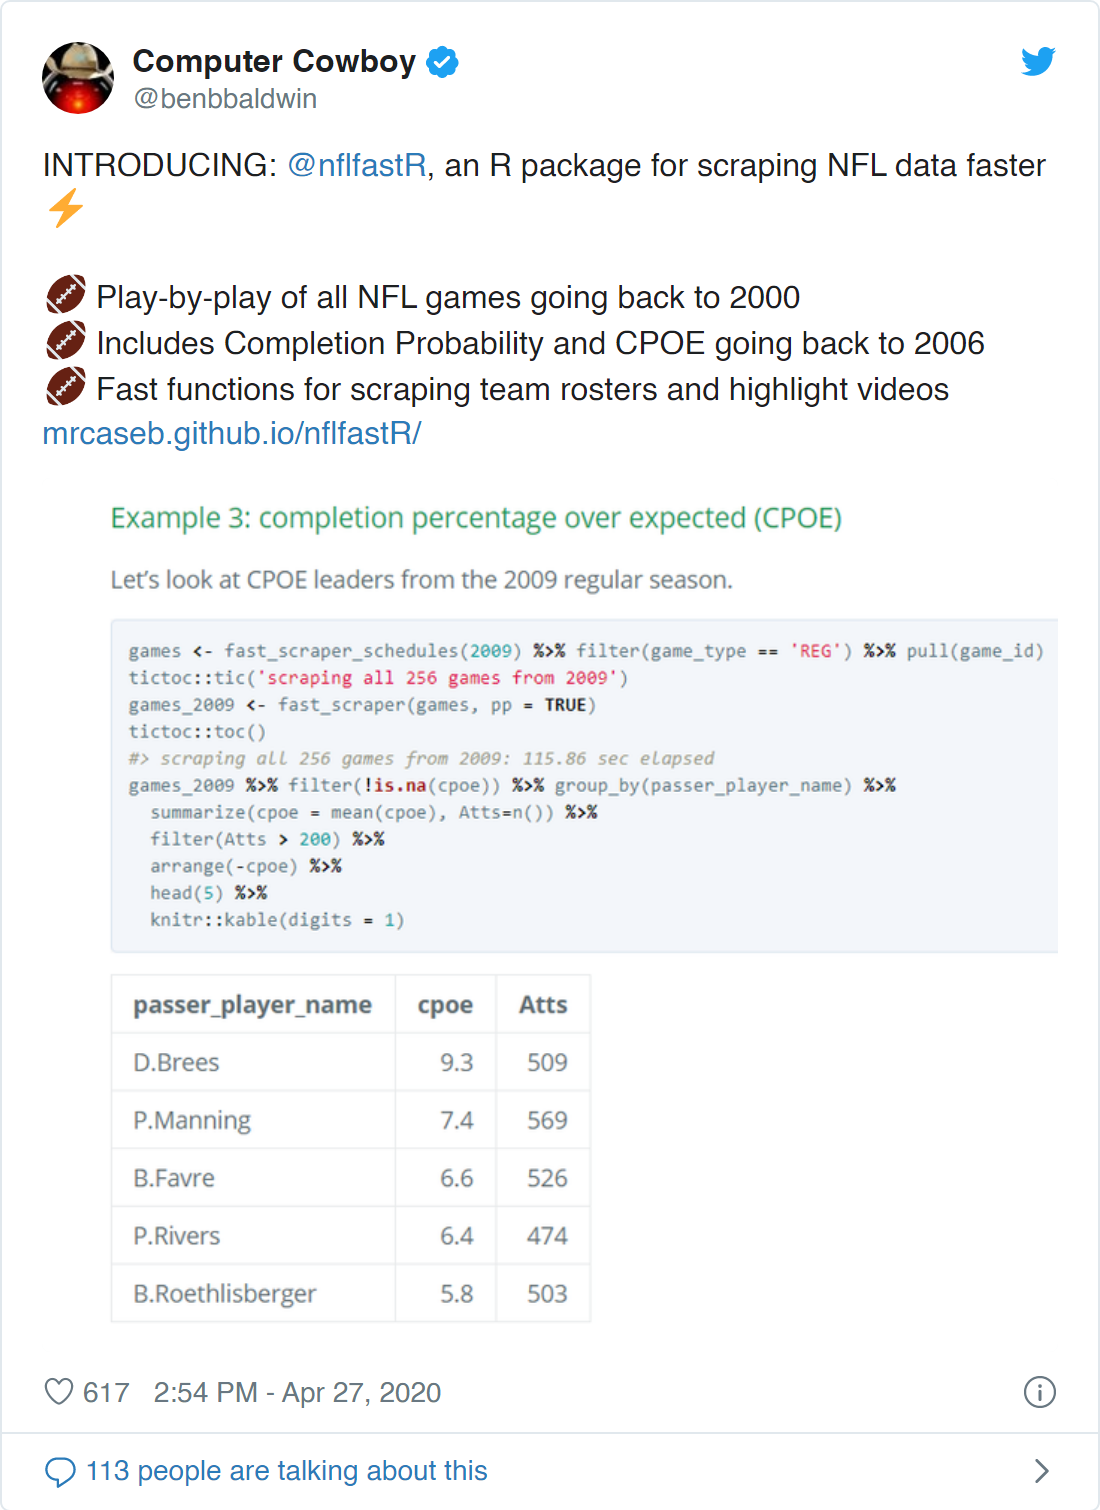
\includegraphics[width=1\textwidth,height=\textheight]{./index_files/figure-pdf/ben-baldwin-tweet-1.png}

Thanks to the work of multiple people
(\href{https://twitter.com/mrcaseb}{@mrcaseB},
\href{https://twitter.com/benbbaldwin}{@benbbaldwin},
\href{https://twitter.com/_TanHo}{@TanHo},
\href{https://twitter.com/LeeSharpeNFL}{@LeeSharpeNFL}, and
\href{https://twitter.com/thomas_mock}{@thomas\_mock} \ldots{} to just
name a few), the process of getting started with advanced analytics
using NFL data is now easier than ever.

That said, and without getting too far into the weeds of the history
behind it all, the above-mentioned people are responsible in some shape
or form for the current status of the \texttt{nflverse}, which is a
superb collection of data and R-based packages that allows anybody the
ability to access deeply robust NFL data as far back as the 1999 season.

The \texttt{nflverse} as we know it today was initially birthed from the
\texttt{nflscrapR} project, which was started by the Carnegie Mellon
University student and profess duo of
\href{https://twitter.com/bklynmaks?lang=en}{Maksim Horowitz} and
\href{https://twitter.com/stat_sam}{Sam Ventura}. After Horowitz
graduated - and got hired by the Atlanta Hawks - the \texttt{nflscrapR}
package was taken over by fellow CMU student Ron Yorko (who would go on
to receive his Ph.D.~from the Statistics and Data Science program). The
trio's work on \texttt{nflscrapR} ultimately led to a peer-reviewed
paper titled ``\href{https://arxiv.org/pdf/1802.00998.pdf}{nflWAR: A
Reproducible Method for Offensive Player Evaluation in Football.}''
Ultimately, the \texttt{nflscrapR} project came to an end when the
specific .json feed used to gather NFL data changed. At this point, Ben
Baldwin and Sebastian Carl had already built upon the \texttt{nflscrapR}
project's foundations to create \texttt{nflfastR}. Ron officially marked
the end of the \texttt{nflscrapR} era and the beginning of the
\texttt{nflfastR} era with a tweet on September 14, 2020:\footnote{Thanks
  to Ben Baldwin for chatting with me on Discord and providing this
  brief understanding of the backstory.}

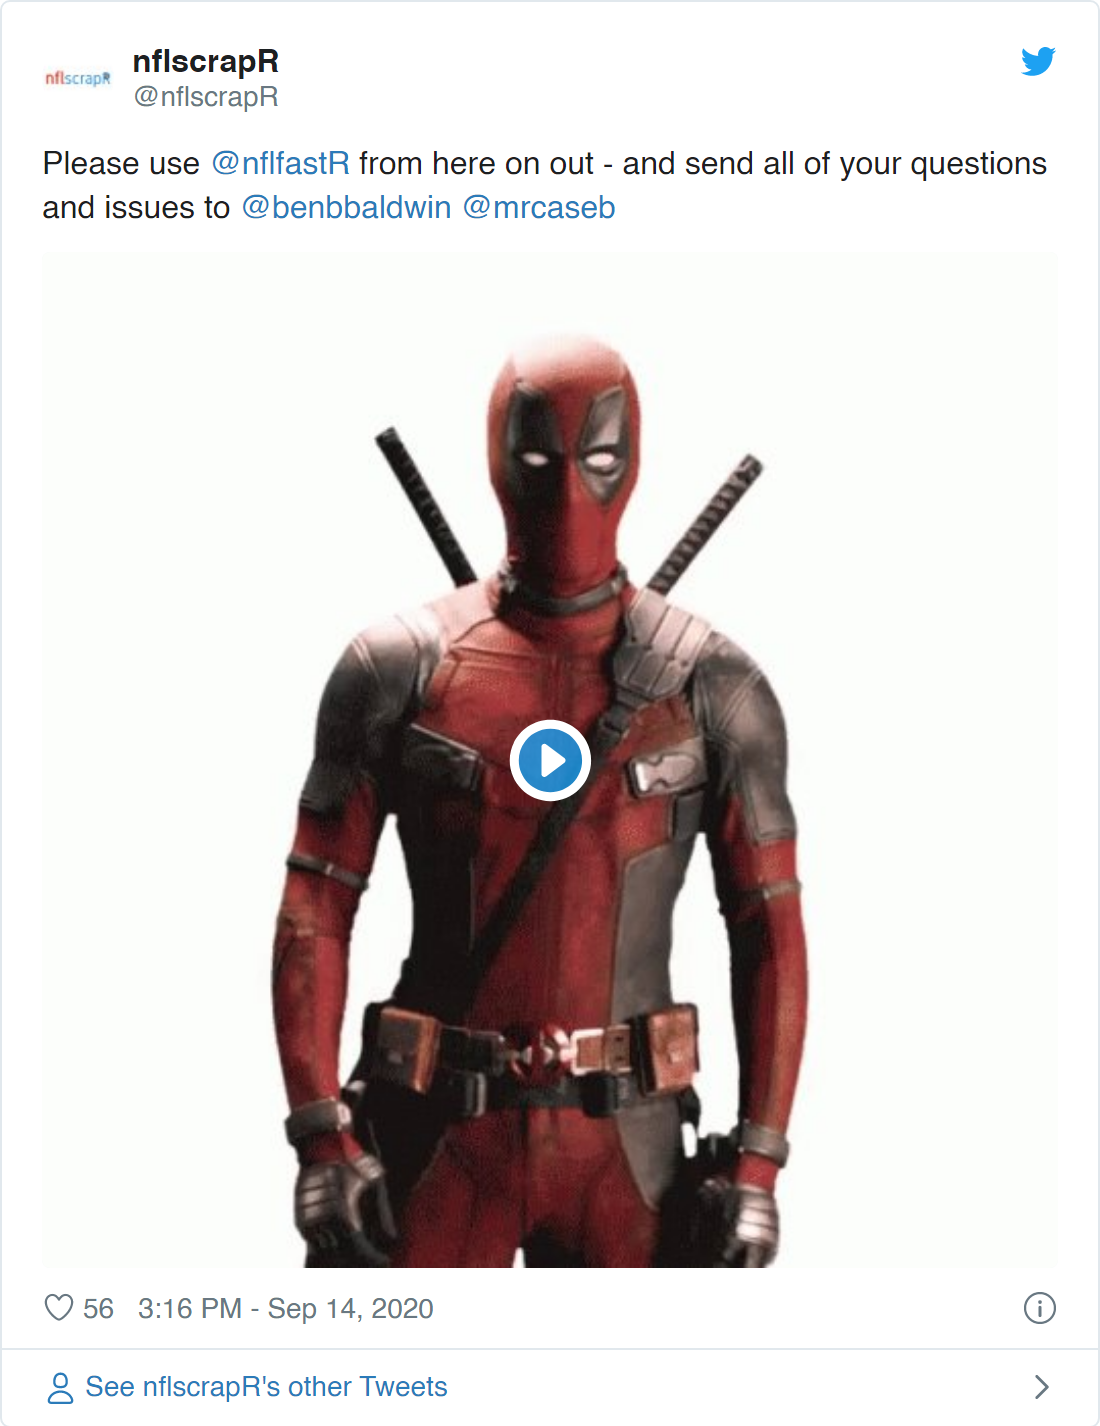
\includegraphics[width=1\textwidth,height=\textheight]{./index_files/figure-pdf/farewell-nflscrapr-tweet-1.png}

As a reply to his first tweet about the \texttt{nflfastR} project, Ben
explained that he created the original function to scrape NFL data for
the creation of his \href{https://rbsdm.com/stats/stats/}{NFL analytics
website}. Thankfully, he and Seb did not keep the creation to themselves
and released \texttt{nflfastR} to the public. Because of the ``open
source'' nature of R and R packages, a laundry list of companion
packages quickly developed alongside \texttt{nflfastR}. The original
\texttt{nflfastR} package is now part of the larger \texttt{nflverse} of
packages that drive the NFL analytics community on Twitter and beyond.

The creation of the \texttt{nflverse} allowed for anybody interested in
NFL analytics to easily access data, manipulate it to their liking, and
release their visualizations and/or metrics to the wider public. In
fact, it is now a regular occurrence for somebody to advance their R
programming ability because of the \texttt{nflverse} and then go on to
win the Big Data Bowl. As of the 2022 version of the Big Data Bowl, over
``30 participants have been hired to work in data and analytics roles in
sports, including 22 that were hired in football'' ({``Big Data Bowl:
The Annual Analytics Contest Explores Statistical Innovations in
Football,''} n.d.). Most recently, the
\href{https://www.boltsfromtheblue.com/2021/7/9/22570490/chargers-news-nfl-big-data-bowl}{Chargers
hired 2020 participate Alex Stern} and the
\href{https://twitter.com/sethwalder/status/1532721476209627136}{Chiefs
hired Marc Richards}, a member of the winning 2021 team, as a Football
Research Analyst.

Kevin Clark, in a 2018 article for
\href{https://www.theringer.com/nfl/2018/12/19/18148153/nfl-analytics-revolution}{\emph{The
Ringer}}, explained that despite not being as obvious as the
sabermetrics movement in baseball, the analytics movement in the NFL is
``happening in front of you all the time.'' The use of analytics in the
NFL did, however, predate Clark's article. In 2014, Eagles head coach
Doug Pederson explained that all decisions made by the organization -
from game planning to draft strategy - were to be informed by hard data
and analytics. Leading this early adoption of analytics, and reporting
directly to team Vice President Howie Roseman, were Joe Douglas and Alec
Halaby, ``a 31-year-old Harvard grad with a job description'' that had
an emphasis on ``integrating traditional and analytical methods in
football decision-making.'' The result? A ``blending of old-school
scouting and newer approaches'' that were often only seen in other
leagues, such as the NBA and MLB (Rosenthal 2018). Pederson believed in
and trusted the team's approach to analytics so much that a direct line
of communication was created between the two during games, with the
analytics department providing the head coach with math-based
recommendations for any scenario Pederson requested (Awbrey
2020).\footnote{Thanks, again, to Ben Baldwin for providing his personal
  knowledge about the ``early days'' of the Eagles' analytics
  department.}

In just under five years time since the publishing of that article, it
has become hard to ignore the analytic movement within the NFL. Yet,
there is still so much growth to happen in the marriage between the NFL
and advanced metrics. For example, there is no denying that the
sabermetrics movement drastically ``altered baseball's DNA'' Heifetz
(2019){]}. Moreover, as explained in Seth Partnow's outstanding
\href{https://www.amazon.com/Midrange-Theory-Basketballs-Evolution-Analytics/dp/1637270968/ref=tmm_pap_swatch_0?_encoding=UTF8\&qid=1656245879\&sr=8-4}{\emph{The
Midrange Theory: Basketball's Evolution in the Age of Analytics}}, the
analytics movement in the NBA essentially killed the midrange shot
(briefly: it is more beneficial to try to work the ball in directly
under the basket (for a high-percentage shot) or to take the 3-pointer,
as the possible additional point is statistically worth more despite the
lower success probability as opposed a 2-point midrange shot) as well as
the traditional, ``old-school'' center position.

Compared to both the NBA and MLB, the NFL is playing catch up in
analytics driving changes equivalent to the death of the midrange shot
or the plethora of additional tactics and changes to baseball because of
sabermetrics. Joe Banner, who served as the President of the Eagles from
2001-2012 and then the Chief Executive Officer of the Browns from
2012-2013, explained that some of the hesitation to incorporate
analytics into NFL game planning was a result of the game being ``very
much driven by conventional wisdom to an extreme degree'' (Fortier
2020). Perhaps nobody encapsulates this better than Pittsburgh Steelers
Head Coach Mike Tomlin. When asked about his position on analytics
during the 2015 season, Tomlin explained:

\begin{quote}
I think that's why you play the game. You can take analytics to baseball
and things like that but football is always going to be football. I got
a lot of respect for analytics and numbers, but I'm not going to make
judgements based on those numbers. The game is the game. It's an
emotional one played by emotional and driven men. That's an element of
the game you can't measure. Often times decisions such as that weigh
heavily into the equation (Kozora 2015).
\end{quote}

Given that Tomlin's quote is from 2015, perhaps the Steelers pivoted
since and are now more analytically inclined. That does not seem to be
the case. In a poll of NFL analytics staffers conducted by ESPN,
\href{https://www.espn.com/nfl/story/_/id/29939438/2020-nfl-analytics-survey-which-teams-most-least-analytically-inclined\#least}{the
Steelers were voted as one of the least analytically advanced teams in
the league.}

There is large gap between the least analytically inclined teams
(Washington, Tennessee, Cincinnati, New York Giants, and Pittsburgh) and
those voted as the most analytically inclined (Baltimore, Cleveland,
Philadelphia, and Houston). In the ESPN poll, the Browns were voted as
the analytics department producing the highest level of work. One of
those polled spoke to the fact that much of this outstanding work is a
result of General Manager Andrew Berry being a ``true believer,''
explaining that he is one of the ``rare guys you'll come across in life
where you think to yourself, `Man, this guy thinks at a different level.
Just pure genius.' He's one of them.''

\href{https://www.washingtonpost.com/sports/2020/01/16/nfls-analytics-movement-has-finally-reached-sports-mainstream/}{In
his article for the \emph{Washington Post}}, Sam Fortier argues that
many teams became inspired to more intimately introduce analytics into
game planning and on-field decisions after the 2017 season. On their run
to becoming Super Bowl Champions, the Philadelphia Eagles were
aggressive on 4th down, going for it 26 times during the season and
converting on 17 of those for a conversion percentage of 65.4\%. A quick
examination and visualization of data highlights the absolutely
staggering increase in 4th aggressiveness among NFL head coaches from
2017-2021:

\begin{figure}

{\centering 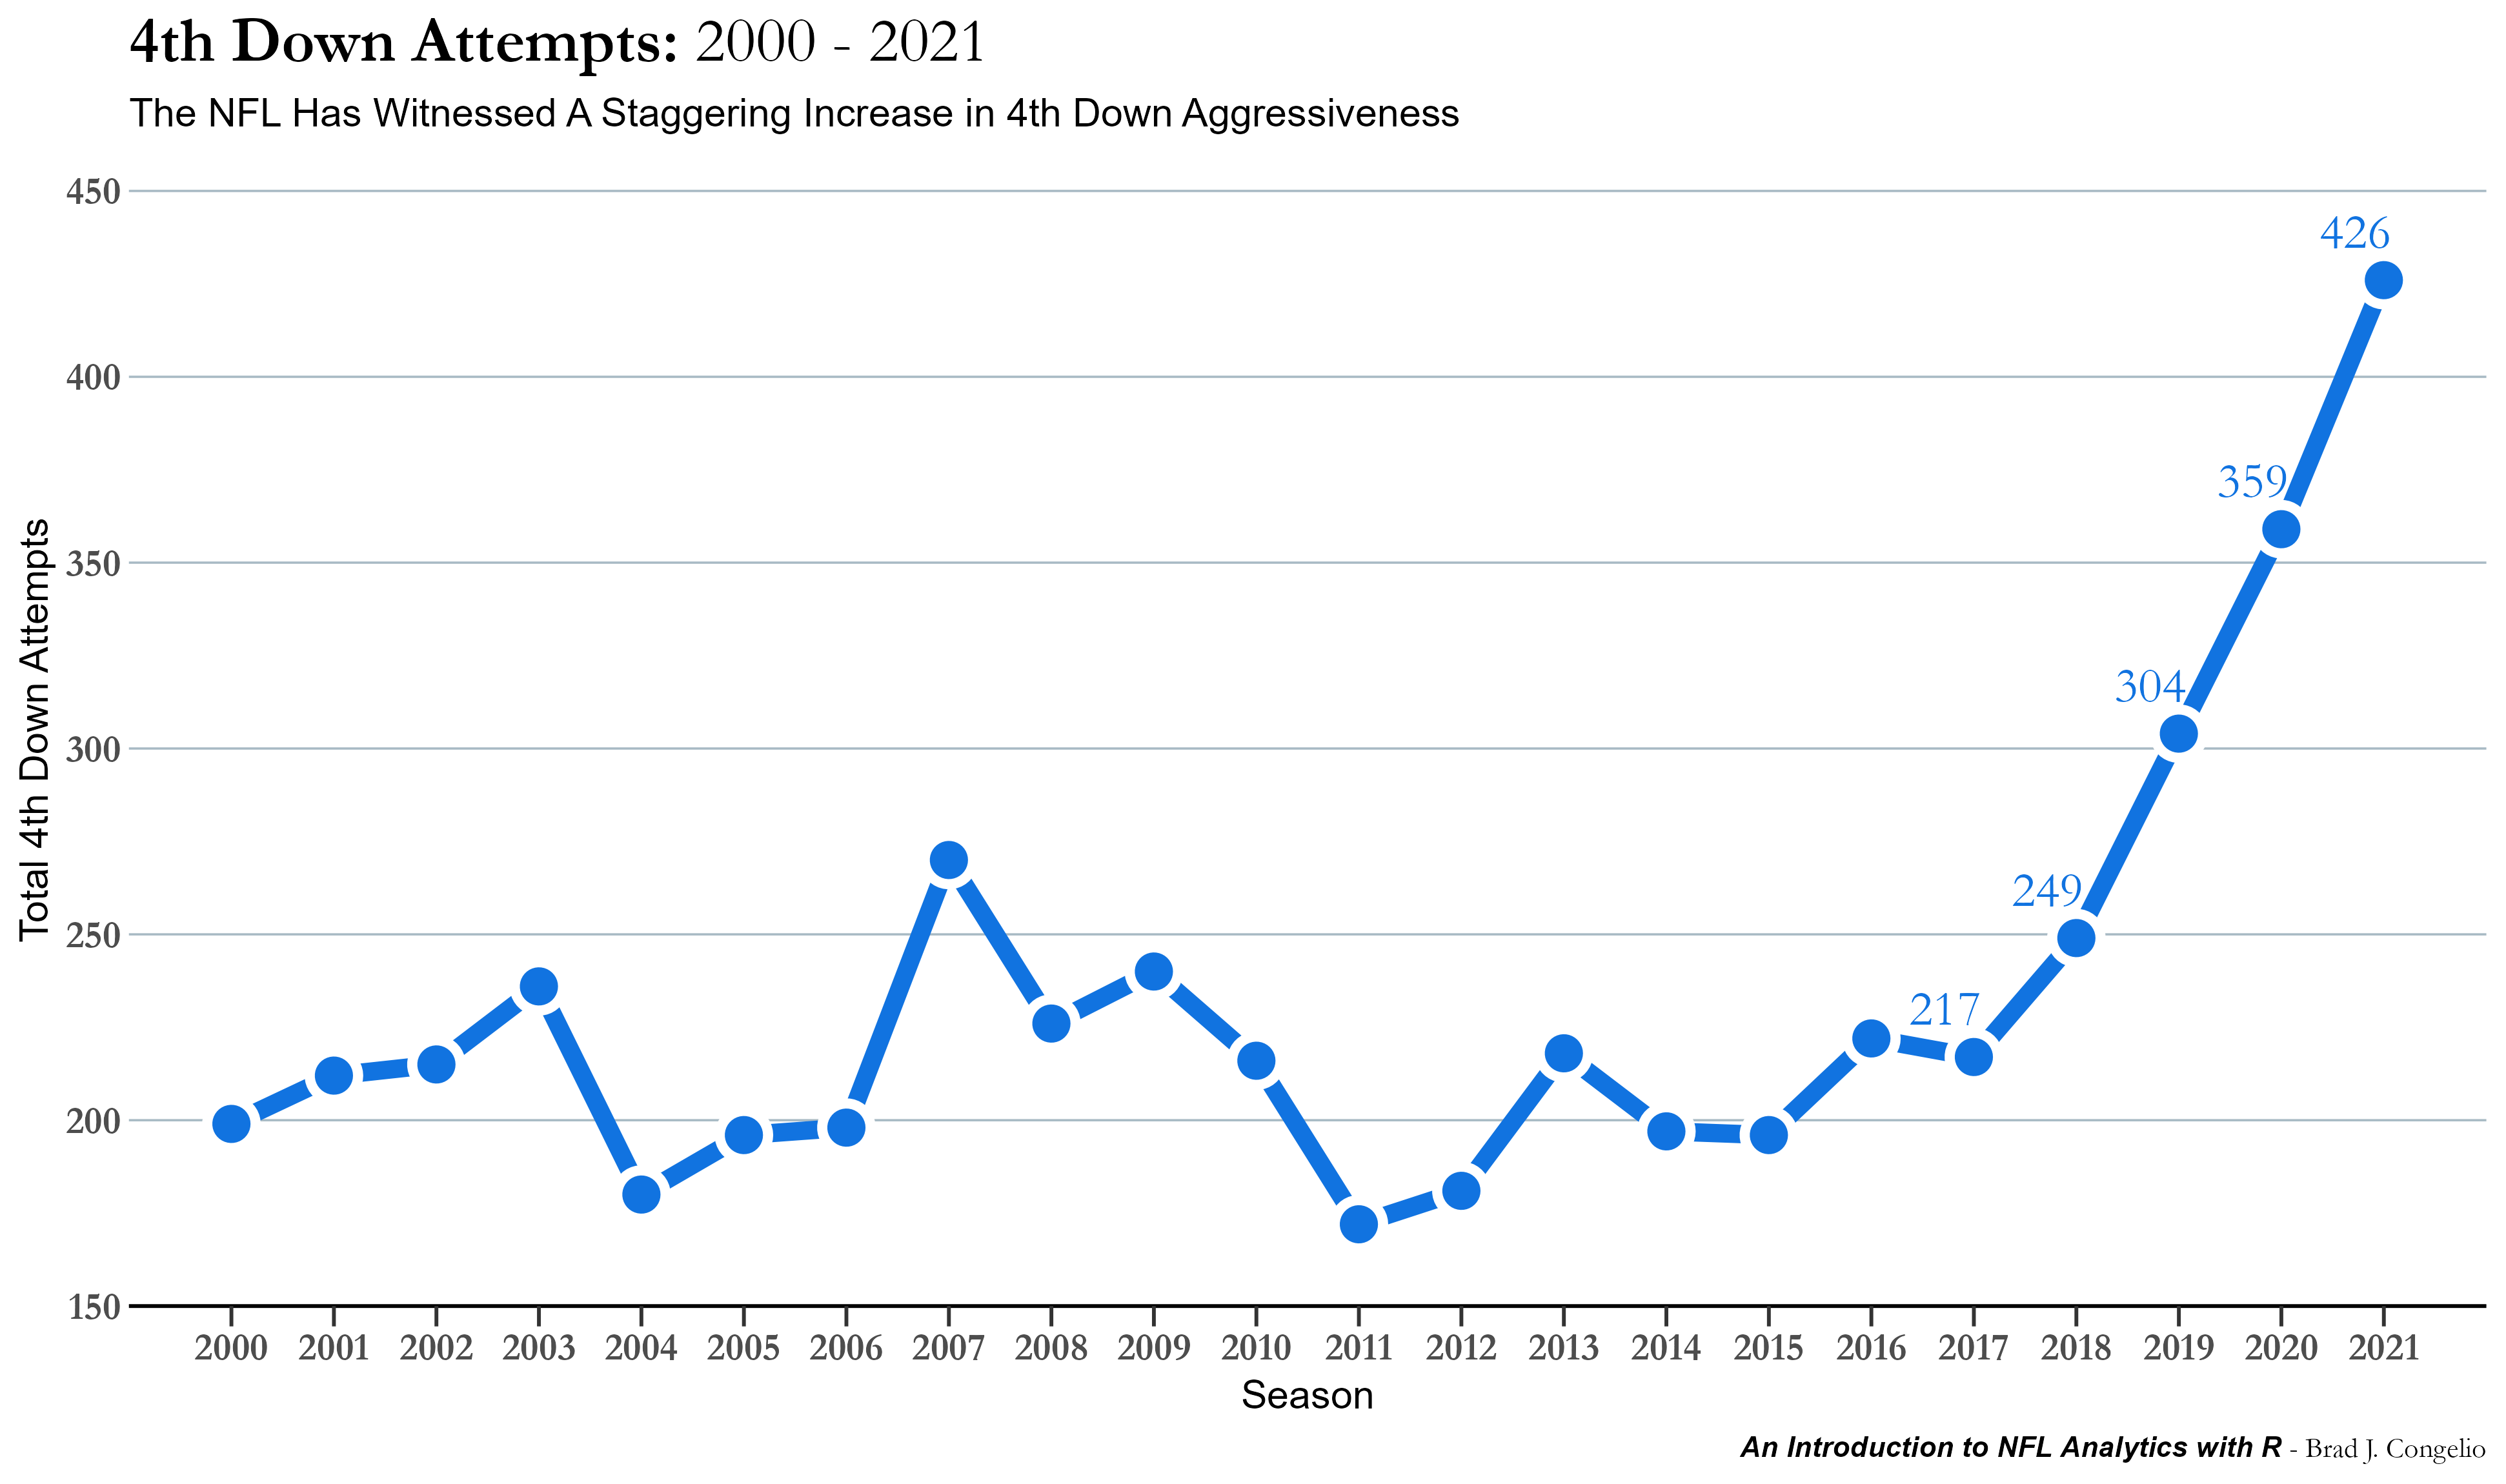
\includegraphics[width=1\textwidth,height=\textheight]{./images/4th-down-attempts.png}

}

\caption{4th Down Attempts: 2000 - 2021}

\end{figure}

There has been a 96.3\% increase in the number of 4th down attempts from
just 2017 to 2021. In fact, the numbers may actually be higher as I was
quite conservative in building the above plot by only considering those
4th down attempts that took place when the offensive team had between a
5-to-95\% winning probability and those prior to the two-minute warning
of either half. Even with those conservative limitations, the increase
is staggering. The numbers, however, support this aggression. During
week one of both the 2020 and 2021 season, \emph{not} going for it on
4th down ``cost teams a cumulative 170 percentage points of win
probability'' (Bushnell 2021).

Ben Baldwin, using the \texttt{nfl4th} package that is part of the
\texttt{nflverse}, tracked the shift in NFL coaching mentality regarding
4th down decisions by comparing 2014's ``go for it percentage'' against
the same for 2020. When compared to the 2014 season, NFL coaches are now
much more in agreement with analytics on when to ``go for it'' on 4th
down in relation to the expected gain in win probability.

\begin{figure}

{\centering \includegraphics[width=1\textwidth,height=\textheight]{./images/baldwin-graph-goforit.png}

}

\caption{Credit: Ben Baldwin}

\end{figure}

It should not be surprising then, considering Mike Tomlin's quote from
above and other NFL analytics staffers voting the Steelers as one of the
least analytically driven teams in the league, that Pittsburgh lost the
most win probability by either kicking or punting in ``go for it''
situations during the 2020 NFL season. On the other end, the Ravens and
Browns - two teams voted as the most analytically inclined - are the two
best organizations at knowing when to ``go for it'' on 4th down based on
win probability added. There seems to be a defined relationship between
teams buying into analytics and those who do not:

\begin{figure}

{\centering \includegraphics[width=1\textwidth,height=\textheight]{./images/tomlin-go-for-it.png}

}

\caption{Credit: Ben Baldwin}

\end{figure}

The NFL's turn towards more aggressive 4th-down decisions is just one of
the many analytics-driven changes occurring in the league. Another
significant example is Defense-Adjusted Value over Average (or DVOA), a
formula created by Aaron Schatz, now the editor in chief of
\href{https://www.footballoutsiders.com/info/methods\#dvoa}{Football
Outsiders}, that sought to challenge the notion that teams should,
first, establish the running game in order to open up the passing game.
Some of these changes are apparent on televisions screens on Sunday
afternoons in the Fall, while others are occurring behind the scenes
(analytics departments working on scouting and draft preparation, for
example). Indeed, the use of analytics in the NFL is not as tightly
ingrained as we see in other prominent leagues. And we must remember
that there are certainly continued hold outs among some NFL coaches
(like Mike Tomlin).

Despite some coaching hold outs on fully embracing analytics, the
``thirst for knowledge in football is as excessive as any other sport
and the desire to get the most wins per dollar is just as high.'' As the
pipeline of data continues to grow, both internally in the league and
data that becomes publicly accessible, ``smart teams will continue to
leave no rock unturned as they push the limits on how far data can take
them.'' Joe Banner explained that while the NFL has long been a league
of coaches saying ``well, that is the way we've always done it,'' the
league is ripe for a major shift (Bechtold 2021).

Banner's belief that those teams searching for every competitive
advantage will ``leave no rock unturned'' is the driving force behind
this book. For all intents and purposes, the age of analytics in the NFL
is still in its infancy. Turning back, again, to the 2017 season, the
Eagles' management praised and credited the team's analytics department
as part of the reason they were able to win Super Bowl LII. Doing so
Danney Heifetz argues, ``changed the language of football.'' The NFL, he
explains, is a ``copycat league'' and, as witnessed with the increase in
4th down aggressiveness since 2017, teams immediately began to carbon
copy Philadelphia's approach to folding traditional football strategy
with a new age analytics approach. Because of the modernity of this
relationship between long-held football dogmas and analytics, nobody can
be quite sure what other impacts it will create on the gamesmanship of
football.

However, as Heifetz opines, both the NBA and MLB can serve as a roadmap
to where analytics will take the NFL. Importantly, the NFL's
relationship with analytics is still in its ``first frontier of what
will likely be a sweeping change over the next two decades.'' Because of
this, we cannot be sure what the next major impact analytics will make,
nor when it may occur. But, with the ever-growing amount of publicly
accessible data, it is only a matter of time until it is discovered. For
example, in an interview with Heifetz, Brian Burke - one of the
forefather's of NFL analytics and now a writer for ESPN - expressed his
belief that the next major impact will be ``quantifying how often
quarterbacks make the correct decision on the field.''

It seems that every new NFL season results in an amateur analyst
bringing a groundbreaking model and/or approach to the table. Unlike,
for example, MLB where there is little left to discover in terms of
sabermetrics and new approaches to understanding the game and its
associated strategy, the NFL is - for lack of a better phrase - an open
playing field. With more and more data becoming available to the public,
it is now easier than ever investigate your own ideas and suspicions and
to create your own models to confirm your intuition.

For example, I am originally from the greater Pittsburgh area and am a
big Steelers fan (which certainly explains some of the Steelers-centric
examples I use in the writing of this book). I was adamant in my belief
that Pittsburgh's TJ Watt should win the 2021 Defensive Player of the
Year award, despite many others calling for Los Angeles' Aaron Donald to
claim the title. In effort to prove my point, I sought out to design
what I coined \textbf{\emph{Adjusted Defensive Impact}}. To begin, I
wanted to explore the idea that not all defensive sacks are created
equal, as a player's true impact is not always perfectly represented by
top-level statistics.

To account for that, I opted to adjust and add statistical weight to
sack statistics. This was done over multiple areas. For instance, not
all players competed in all 17 regular-season games in 2021. To adjust
for this, I took the total of game played in the data (2,936) and
divided by 17 (a full season) to achieve a weighted adjustment of
0.0058. TJ Watt played in just 15 games in 2021. His adjusted equation,
therefore, is (17-`games') * 0.0058. The result? He gets a bit more
credit for this adjustment than, say, Myles Garrett who played all 17
regular-season games.

Going further with the model, I created a weighted adjustment for solo
sacks (0.90), a negative weighted adjustment (-0.14) for any sack
charted as ``unblocked,'' and a weighted adjustment to account for how
many times a player actually rushed the QB compared to how many
defensive snaps they played. Using data from the SIS Data Hub, the full
code is below:

\begin{Shaded}
\begin{Highlighting}[]
\FunctionTok{options}\NormalTok{(}\AttributeTok{digits =} \DecValTok{2}\NormalTok{)}

\DocumentationTok{\#\# selecting just information I want and then renaming}
\NormalTok{pass.data }\OtherTok{\textless{}{-}}\NormalTok{ pass\_rush\_data }\SpecialCharTok{\%\textgreater{}\%}
  \FunctionTok{select}\NormalTok{(Player, Team, Games, }\StringTok{\textasciigrave{}}\AttributeTok{Pass Snaps}\StringTok{\textasciigrave{}}\NormalTok{, }\StringTok{\textasciigrave{}}\AttributeTok{Pass Rushes}\StringTok{\textasciigrave{}}\NormalTok{,}
         \StringTok{\textasciigrave{}}\AttributeTok{Solo Sacks}\StringTok{\textasciigrave{}}\NormalTok{, }\StringTok{\textasciigrave{}}\AttributeTok{Ast. Sacks}\StringTok{\textasciigrave{}}\NormalTok{, }\StringTok{\textasciigrave{}}\AttributeTok{Comb. Sacks}\StringTok{\textasciigrave{}}\NormalTok{, }
         \StringTok{\textasciigrave{}}\AttributeTok{Unblocked Sacks}\StringTok{\textasciigrave{}}\NormalTok{, Hurries, Hits) }\SpecialCharTok{\%\textgreater{}\%}
  \FunctionTok{rename}\NormalTok{(}\AttributeTok{total.snaps =} \StringTok{\textasciigrave{}}\AttributeTok{Pass Snaps}\StringTok{\textasciigrave{}}\NormalTok{,}
         \AttributeTok{total.rushes =} \StringTok{\textasciigrave{}}\AttributeTok{Pass Rushes}\StringTok{\textasciigrave{}}\NormalTok{,}
         \AttributeTok{solo.sacks =} \StringTok{\textasciigrave{}}\AttributeTok{Solo Sacks}\StringTok{\textasciigrave{}}\NormalTok{,}
         \AttributeTok{asst.sacks =} \StringTok{\textasciigrave{}}\AttributeTok{Ast. Sacks}\StringTok{\textasciigrave{}}\NormalTok{,}
         \AttributeTok{comb.sacks =} \StringTok{\textasciigrave{}}\AttributeTok{Comb. Sacks}\StringTok{\textasciigrave{}}\NormalTok{,}
         \AttributeTok{unblocked.sacks =} \StringTok{\textasciigrave{}}\AttributeTok{Unblocked Sacks}\StringTok{\textasciigrave{}}\NormalTok{,}
         \AttributeTok{player =}\NormalTok{ Player,}
         \AttributeTok{team =}\NormalTok{ Team,}
         \AttributeTok{games =}\NormalTok{ Games,}
         \AttributeTok{hurries =}\NormalTok{ Hurries,}
         \AttributeTok{hits =}\NormalTok{ Hits)}

\DocumentationTok{\#\# creating a new column to get percentages of snaps where player rushed}
\NormalTok{pass.data}\SpecialCharTok{$}\NormalTok{rush.percent }\OtherTok{\textless{}{-}}\NormalTok{ pass.data}\SpecialCharTok{$}\NormalTok{total.rushes }\SpecialCharTok{/}\NormalTok{ pass.data}\SpecialCharTok{$}\NormalTok{total.snaps}

\DocumentationTok{\#\# getting weights to add to the equation}
\DocumentationTok{\#\# for example, a solo sack is "more impressive" than an assisted sack. }
\DocumentationTok{\#\# to account for this, we will take the sum of combined sacks (995) and divide }
\DocumentationTok{\#\# by the sum of solo sacks (892) which is (0.9). Therefore, a weight of 0.9 will}
\DocumentationTok{\#\# be placed on solo sacks.}

\DocumentationTok{\#\# as well, a negative weight will be applied to unblocked sacks. Using the total}
\DocumentationTok{\#\# of solo sacks (892) and dividing by the sum of unblocked sacks (128) gives us a}
\DocumentationTok{\#\# NEGATIVE weight of 0.14 to be applied to unblocked sacks}

\DocumentationTok{\#\# further, a weight must be applied to those players who played less than a complete season.}
\DocumentationTok{\#\# the weight here works out to be 0.0058.}

\DocumentationTok{\#\# summarizing information}
\NormalTok{calculated.impact }\OtherTok{\textless{}{-}}\NormalTok{ pass.data }\SpecialCharTok{\%\textgreater{}\%}
  \FunctionTok{group\_by}\NormalTok{(player) }\SpecialCharTok{\%\textgreater{}\%}
  \FunctionTok{summarize}\NormalTok{(}
    \AttributeTok{adjusted.games =}\NormalTok{ (}\DecValTok{17} \SpecialCharTok{{-}}\NormalTok{ games) }\SpecialCharTok{*} \FloatTok{0.0058}\NormalTok{,}
    \AttributeTok{adjusted.solo =}\NormalTok{ solo.sacks }\SpecialCharTok{*} \FloatTok{0.9}\NormalTok{,}
    \AttributeTok{adjusted.unblocked =}\NormalTok{ unblocked.sacks }\SpecialCharTok{/} \SpecialCharTok{{-}}\FloatTok{0.14}\NormalTok{,}
    \AttributeTok{adjusted.rush.percent =} \FloatTok{0.81} \SpecialCharTok{{-}}\NormalTok{ rush.percent,}
    \AttributeTok{combined.impact =} \FunctionTok{sum}\NormalTok{(adjusted.games }\SpecialCharTok{+}\NormalTok{ (solo.sacks }\SpecialCharTok{*} \FloatTok{0.9}\NormalTok{) }\SpecialCharTok{+}\NormalTok{ (unblocked.sacks }\SpecialCharTok{*} \SpecialCharTok{{-}}\FloatTok{0.14}\NormalTok{) }\SpecialCharTok{+}\NormalTok{ adjusted.rush.percent))}
\end{Highlighting}
\end{Shaded}

The end result? Taking into account the above adjusted defensive impact,
TJ Watt was absolutely dominant during the 2021 season:

\begin{figure}

{\centering 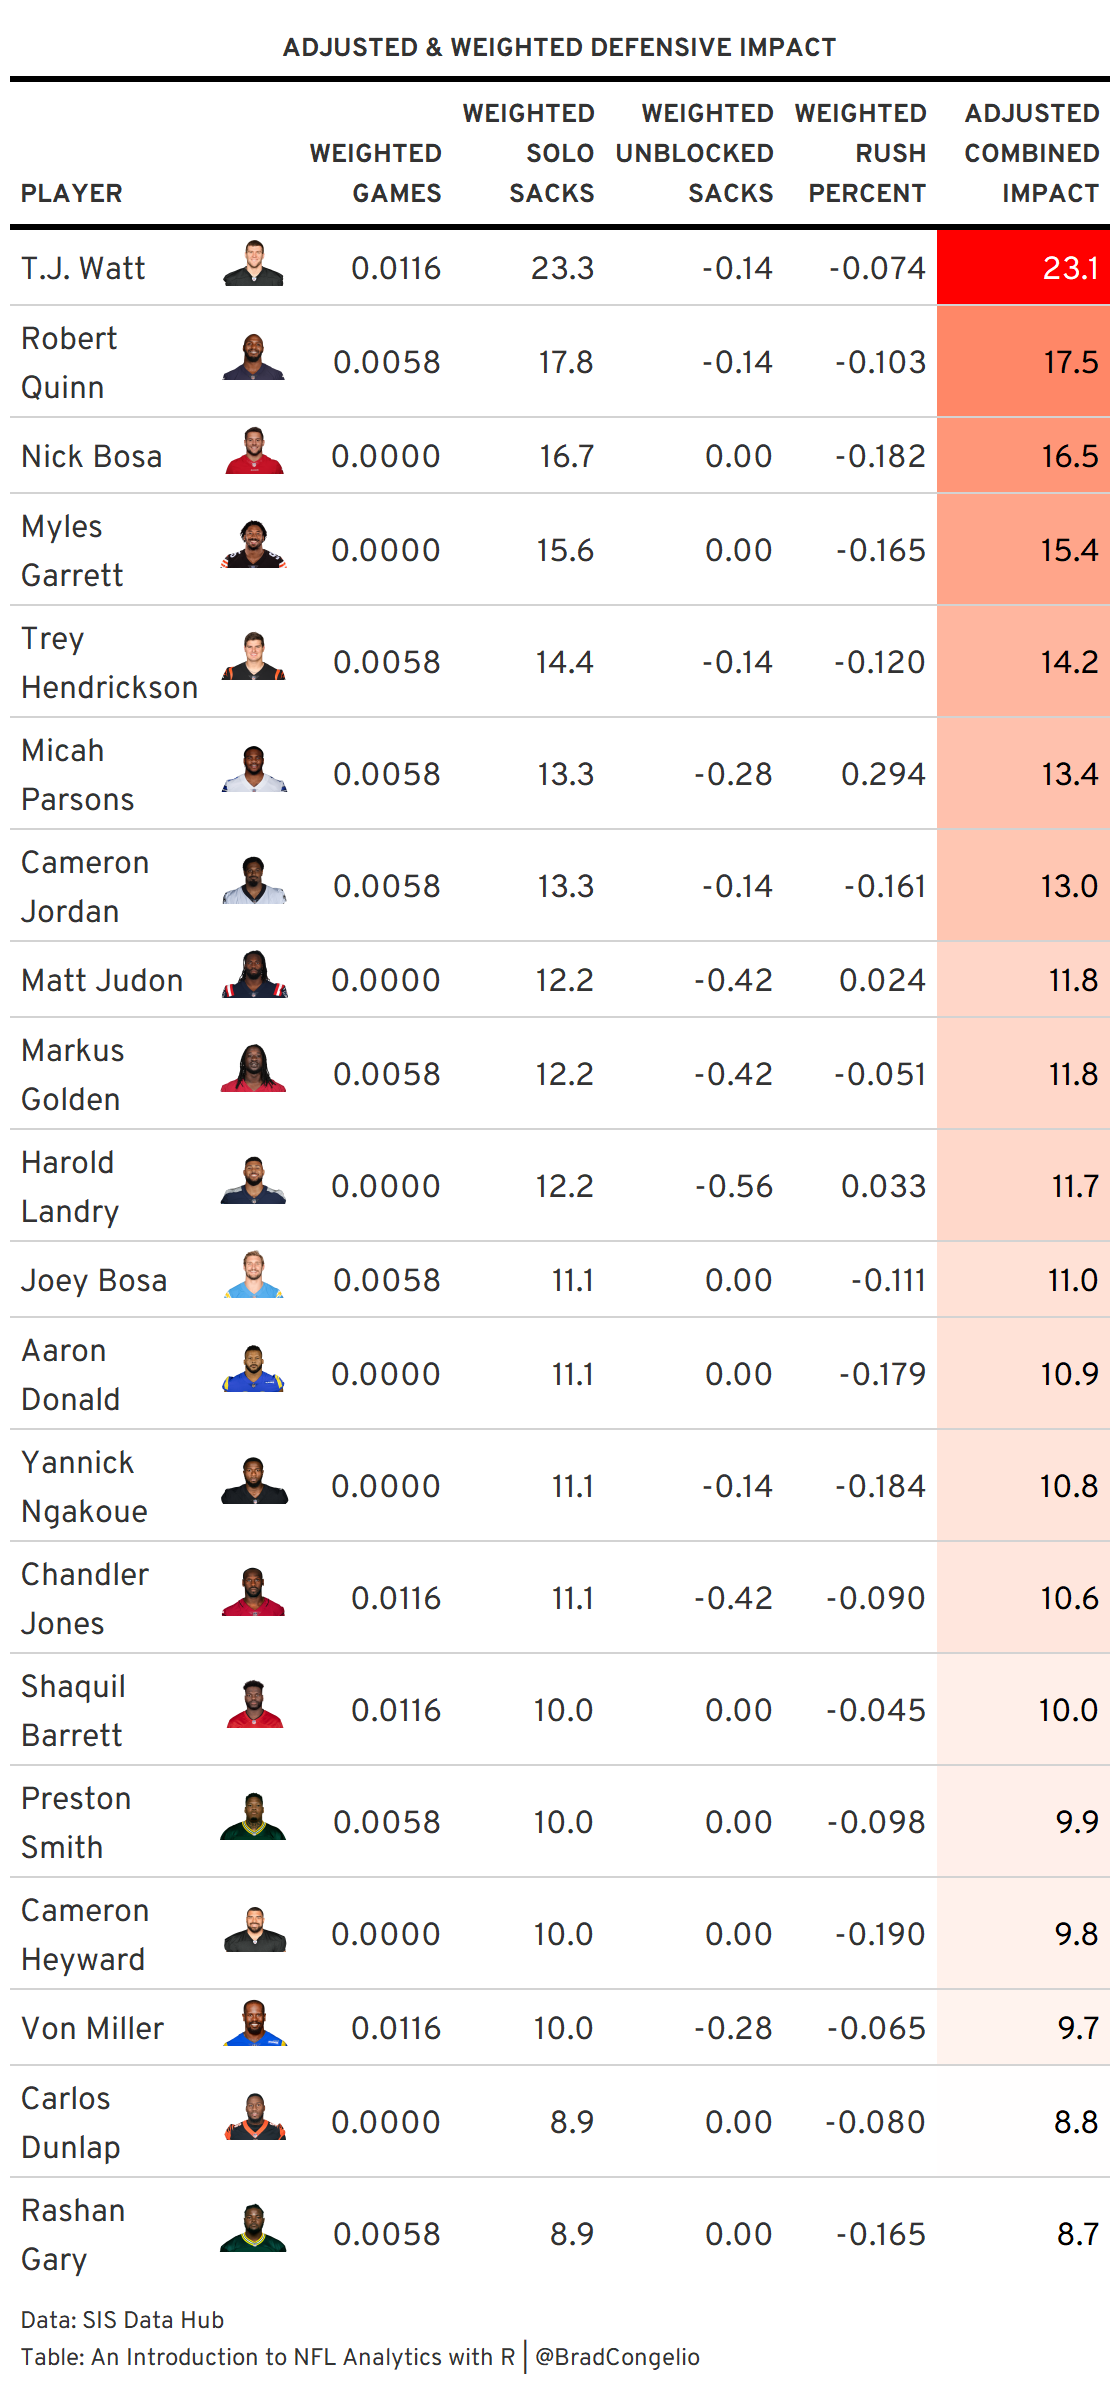
\includegraphics[width=1\textwidth,height=\textheight]{./images/adjusteddefense.png}

}

\caption{Adjusted Defensive Impact}

\end{figure}

All of these examples - from Ben Baldwin's 4th-down model, to Football
Outsiders' DVOA, to my attempt to further quantify defensive player
impact - are just the leading edge of the burgeoning analytics movement
in the NFL. Moreover, the beauty of analytics is that you do not have to
be a mathematician or statistics buff in order to enter the fray. All it
takes is a genuine curiosity to explore what Bob Carroll, Pete Palmer,
and John Thorn coined as the ``\href{https://amzn.to/3y1GZTO}{Hidden
Game of Football}'' and the desire to learn, if you have not already,
the R programming language.

\hypertarget{who-this-book-is-for}{%
\subsection{Who This Book Is For}\label{who-this-book-is-for}}

Writing a book that is wholly dependent on the R programming language to
achieve the end goals is not an easy task, as there are likely two types
of people reading this: those with familiarity in R and those without.
If you are part of the former group, you can likely skip chapter 2 as it
is a primer on installing R and learning the language of the
\texttt{tidyverse}. On the other hand, if you are part of the latter
group, you should skip ahead to chapter 2 before even looking at chapter
1, which serves as an introduction to the \texttt{nflverse} with
examples. That said, this book can serve multiple audiences:

\begin{enumerate}
\def\labelenumi{\arabic{enumi}.}
\item
  Those interested in learning how to produce NFL analytics regardless
  of their current knowledge of the R programming language.
\item
  Professors who instruct data science courses can provide lessons
  through the lens of sport or, perhaps better, create their own Sport
  Analytics courses designed around the book. Moreover, future plans for
  this book include instruction reference guides to include PowerPoint
  templates, assignments/project instructions and grading rubrics, and
  quiz/exam content for online management systems (D2L, Canvas, Moodle,
  etc.).
\item
  Students are able to use this book in multiple ways. For example, in
  my Sport Analytics course, students are first introduced to R and the
  \texttt{tidyverse} using the built-in R data sets (\texttt{mtcars},
  \texttt{iris}, and \texttt{nycflights13}). While those data sets
  certainly serve a purpose, I have found that students grasp the
  concepts and language of the \texttt{tidyverse} more quickly when the
  class turns to using data from the \texttt{nflverse}. Because of this,
  students can use this book to start learning the R programming
  language using football terms (passing yards, first downs, air yards,
  completion percentage over expected) as opposed to the variables they
  may find much less interesting housed in the built-in data. Moreover,
  students already fluid in R can use this book to construct machine
  learning models using football data, for example, as part of
  assignments in data science/analytics courses.
\item
  Journalists, bloggers, and arm-chair quarterbacks alike can use the
  book to underpin their arguments and to provide hard data to backup
  their claims.
\end{enumerate}

It is also important to note that it is not expected for you to be an
expert in statistics, coding, or data modeling in order to find this
book useful. In fact, I self-taught myself the R programming language
after discovering its potential usefulness in my personal academic
research. I only ``became more serious'' about advancing my
understanding of the language's nuances, and more advanced methods,
after discovering the \texttt{nflscrapR} package and using it as my
learning tool for the deep dive into R. My decision to pursue an
academic certificate in the language was driven by the creation of my
Sport Analytics course, as the certificate provided the ``academic
training'' proof that was necessary to move the course through the
University's curriculum committee. Nonetheless, because of this
self-taught journey - and despite being an academic myself - I find that
I largely avoid the use of ``complicated jargon'' that is so evident in
most formal writing.

Because of this, and regardless of which chapter you begin with, I
believe that this book achieves its main goal: to provide a gentle
introduction to doing NFL analytics with R.

\hypertarget{overview-of-chapters}{%
\section{Overview of Chapters}\label{overview-of-chapters}}

\begin{itemize}
\item
  \textbf{Chapter 1} provides an overview of the \texttt{nflverse} with
  specific attention paid to the difference between using
  \texttt{nflfastR} versus \texttt{nflreadr}. Serving as the first dive
  into analytics, the chapter showcases how to use \texttt{nflreadr} to
  retrieve both compiled weekly NFL stats and the deeply robust
  play-by-play statistics. In both cases, exercises are provided.
  Readers will do their first coding by, first, using the weekly stats
  to determine the 2021 leaders in air yards per attempt. Second,
  readers will use the play-by-play statistics from the 2021 season to
  create a brand new metric (QB aggressiveness on 3rd down pass
  attempts). Afterward, readers will learn how to retrieve multiple
  seasons of data at once.
\item
  \textbf{Chapter 2} covers the process of downloading both R and
  RStudio, as well as the necessary packages to do NFL analytics. As one
  of the most important chapters in the book (especially for those new
  to the R programming language), readers take a deep dive into
  wrangling NFL data with the \texttt{tidyverse} package. To begin,
  readers will learn about the \texttt{dplyr} pipe
  (\texttt{\%\textgreater{}\%}) and use, in exercises, the six most
  important verbs in the \texttt{dplyr} language: \texttt{filer()},
  \texttt{select()}, \texttt{arrange()}, \texttt{summarize()},
  \texttt{mutate()}, and \texttt{group\_by()}. At the conclusion of the
  chapter, multiple exercises are provided to allow readers to practice
  using the \texttt{dplyr} verbs, relational operators within the
  \texttt{filter()} function and creating ``new stats'' by using the
  \texttt{summarize()} function. Moreover, readers will determine the
  relationship between the \texttt{dplyr} language and important
  variables within the \texttt{nflverse} data such as
  \texttt{player\_name} and \texttt{player\_id}, which is important for
  correct manipulation and cleaning of data.
\item
  \textbf{Chapter 3} examines the numerous and, often, bewildering
  amount of functions ``underneath the hood'' of the packages that makes
  up the \texttt{nflverse}. For example, \texttt{load\_pbp()} and
  \texttt{load\_player\_stats()} are included in both \texttt{nflfastR}
  and \texttt{nflreadr}. However, \texttt{load\_nextgen\_stats()},
  \texttt{load\_pfr\_stats()}, and \texttt{load\_contracts()} are all
  part of just \texttt{nflreadr}. Because of this complexity, readers
  will learn how to efficiently operate within the \texttt{nflverse}.
  Moreover, chapter 3 provides dozens of examples and exercises related
  to all of the various functions included. For example, readers will
  learn to use \texttt{load\_nextgen\_stats()} to determine which
  running backs get to the line of scrimmage the quickest and will use
  \texttt{load\_pfr\_stats()} to explore advanced defensive metrics
  across multiple seasons.
\item
  \textbf{Chapter 4} moves readers from data cleaning and manipulation
  to an introduction to data visualization using \texttt{ggplot2}. As
  well, chapter 4 provides further instruction on \texttt{nflverse}
  functions such as \texttt{clean\_player\_names()},
  \texttt{clean\_team\_abbrs()}, and \texttt{clean\_homeaway()}. As
  well, to prep for data visualization, readers will be introduced to
  the \texttt{teams\_colors\_logos} and \texttt{load\_rosters} functions
  as well as the \texttt{nflplotR} package, which provides ``functions
  and geoms to help visualization of NFL related analysis'' (Carl 2022).
  Readers will produce multiple types of visualizations, including
  \texttt{geom\_bar}, \texttt{geom\_point}, \texttt{geom\_density}, and
  more. As well, readers will learn to use \texttt{facet\_wrap} and
  \texttt{facet\_grid} to display data over multiple seasons. For
  visualizations that include team logos or player headshots,
  instruction will cover both how to do the coding manually using
  \texttt{teams\_colors\_logos} or \texttt{load\_rosters} and to use the
  \texttt{nflplotr} package to avoid the need to use \texttt{left\_join}
  to merge \texttt{teams\_colors\_logos} to your dataframe.
\item
  \textbf{Chapter 5} introduces advanced methods in R using
  \texttt{nflverse} data, with a specific focus on modeling and machine
  learning. To streamline the process of learning, readers will be
  introduced to \texttt{tidymodels}, a ``collection of packages for
  modeling and machine learning using \texttt{tidyverse} principles''
  (Silge, n.d.). As an example, readers will first be introduced to
  \href{https://twitter.com/tejfbanalytics}{Tej Seth's} Rushing Yards
  Over Expected model (\href{https://github.com/tejseth/RYOE}{GitHub},
  \href{https://mfbanalytics.shinyapps.io/RYOE/}{ShinyApp}). The model
  will serve as a learning tool to help readers understand the
  relationship between \texttt{nflfastR} data and machine learning (in
  Tej's case, an \texttt{xgboost} model). Afterward, specific attention
  is given to binary classification, multiclass classification, and
  regression computer learning models. At the conclusion of the chapter,
  readers will be provided exercises to allow them to develop their own
  supervised and unsupervised machine learning models.
\item
  \textbf{Chapter 6} introduces data from sources outside of the
  \texttt{nflverse}, including premium statistics from Pro Football
  Focus and Sports Info Solutions. Readers will learned to use various
  functions, such as \texttt{clean\_team\_names}, in order to prepare
  the data to merge with data from the \texttt{nflverse}. As well, this
  chapter will introduce readers to working with player tracking data.
  To do so, data will be provided from the
  \href{https://operations.nfl.com/gameday/analytics/big-data-bowl/}{NFL's
  Big Data Bowl}. To highlight the work being completed using player
  tracking, this chapter will discuss the Big Data Bowl entries of
  \href{https://twitter.com/MPloenzke}{Matt Ploenzke}
  (\href{https://operations.nfl.com/media/4204/bdb_ploenzke.pdf}{\emph{The
  Importance of Ball Carrier Downfield Acceleration and Unblocked
  Tackler Distance and Spacing}}) and the team of Kellin Rumsey \&
  Brandon DeFlon
  (\href{https://operations.nfl.com/media/4209/bdb_rumsey_deflon.pdf}{\emph{The
  Battle Between Blocker and Defender Is Often Decided by Leverage}}).
\end{itemize}

\hypertarget{about-the-author}{%
\section*{About The Author}\label{about-the-author}}
\addcontentsline{toc}{section}{About The Author}

I (Bradley Congelio) am currently an Assistant Professor in the College
of Business at \href{https://www.kutztown.edu/}{Kutztown University of
Pennsylvania}. Aside from my core area of instruction, I also instruct
the very popular Sport Analytics (SPT 313) course.

I earned my Ph.D.~from the University of Western Ontario and received a
specialized certificate in R for Data Analytics from the University of
California, San Diego in 2021. I am a proud undergraduate alumni of
\href{https://westliberty.edu/}{West Liberty University} and am a strong
advocate of a broad-based liberal arts education.

My research focuses on using big data, the R programming language, and
analytics to explore the impact of professional stadiums on neighboring
communities. I use the proprietary Zillow ZTRAX database as well as U.S.
Census and other forms of data to create robust, applied, and useful
insight into how best to protect those living in areas where stadiums
are proposed for construction.

As well, my work in sport analytics, specifically the NFL, has been
featured on numerous media outlets, including the \emph{USA Today} and
\emph{Sports Illustrated}.

Finally, my most recent academic, peer-reviewed publications include:

\begin{enumerate}
\def\labelenumi{\arabic{enumi}.}
\item
  Congelio, B. (2022). 'Examining the Impact of New Stadium Construction
  on Local Property Prices Using Data Analytics and the Zillow ZTRAX
  Database.'' \emph{Journal of Business, Economics, and Technology}
  Spring 2022, 39-55.
\item
  Congelio, B. (2021). ``Monitoring the Policing of Olympic Host Cities:
  A Novel Approach Using Data Analytics and the LA2028 Olympic Summer
  Games.'' \emph{Journal of Olympic Studies} 2(2), 129-145.
\item
  Congelio, B. ``Predicting the Impact of a New Stadium on Surrounding
  Neighborhoods Through the Use of a \emph{k}-means Unsupervised
  Clustering Algorithm.'' \uline{Currently under peer review.}
\item
  Congelio, B. ``Examining Megaevent's Impact on Foot Traffic to Local
  Businesses Using Mobility and Demographic Aggregation Data.''
  \uline{Currently under peer review and funded by a \$15,000 grant.}
\end{enumerate}

\hypertarget{why-a-book-instead-of-working-in-analytics}{%
\subsection{Why A Book Instead of Working in
Analytics?}\label{why-a-book-instead-of-working-in-analytics}}

I am sometimes asked why I spend time in the classroom teaching this
material rather than taking my domain knowledge to the ``industry side''
and working in the NFL or an otherwise NFL-connected outlet.

The honest and, likely boring, answer is this: I love teaching. My
favorite experience in the classroom yet is always in my Sport Analytics
course. The frustration and sense of helplessness is palpable in the
first weeks of the semester as students attempt to wrap their head
around, what a former student called, ``this {[}censored{]} foreign
language.'' I insist that they keep pushing through the exercises and
assignments. Often, there is line out my door and extending down the
hallway during office hours comprised of just students from the Sport
Analytics class.

And then something amazing happens.

Typically about halfway through the semester, I start seeing the light
bulbs go off. Instead of cursing in anger at the ``foreign language,''
students begin randomly cursing in excitement as the flow of the
\texttt{tidyverse} language ``clicks.'' Once that happens, it is off to
the races because, once they understand speaking in \texttt{tidyverse},
learning more difficult packages (like \texttt{tidymodels}) seems
doable.

And that is why I teach. That moment where I realize my lecturing,
assisting, explaining, and gentle nudging are all finally paying
dividends - not for me, though. For the students.

This book serves as an extension of that classroom experience. As a
reader of this book, you are now a ``student'' and I hope you do not
hesitate to reach out to me if you ever have any questions or, more
importantly, \emph{when (not if)} you have that ``light bulb moment''
and everything begins to click for you.

\hypertarget{technical-details}{%
\section*{Technical Details}\label{technical-details}}
\addcontentsline{toc}{section}{Technical Details}

This book was written using RStudio's
\href{https://rstudio.github.io/visual-markdown-editing/}{Visual Editor
for R Markdown}. It was published using the \texttt{Quarto} publishing
system built on \texttt{Pandoc}. As well, the following packages were
used in this book:

\begin{table}

\caption{Packages Used In This Book}
\centering
\begin{tabular}[t]{l|l|l}
\hline
package & version & source\\
\hline
dplyr & 1.0.10 & CRAN (R 4.1.3)\\
\hline
ggplot2 & 3.3.6 & CRAN (R 4.1.3)\\
\hline
gt & 0.6.0.9000 & Github (rstudio/gt\textbackslash{}@035c64b0a03f0372750095a7d390edcea4192b91)\\
\hline
nflfastR & 4.4.0.9004 & https://nflverse.r-universe.dev (R 4.1.3)\\
\hline
nflreadr & 1.3.0.03 & Github (nflverse/nflreadr\textbackslash{}@3cfd1576dfdb055356f0a67ab56fadb7b96a57f8)\\
\hline
nflverse & 1.0.2 & https://nflverse.r-universe.dev (R 4.1.3)\\
\hline
scales & 1.2.1 & CRAN (R 4.1.3)\\
\hline
tidymodels & 1.0.0 & CRAN (R 4.1.3)\\
\hline
tidyverse & 1.3.1 & CRAN (R 4.1.1)\\
\hline
webshot & 0.5.2 & CRAN (R 4.1.1)\\
\hline
\end{tabular}
\end{table}

Finally, please note that this book uses the \texttt{dplyr} pipe
operator (\texttt{\%\textgreater{}\%}) as opposed to the new, built-in
pipe operator released with version 4.1 of R
(\texttt{\textbar{}\textgreater{}}). It is likely that you can work
through the exercises and examples in this book by using either
operator. I maintain my use of the \texttt{dplyr} pipe operator for no
other reason than personal preference.

\hypertarget{license}{%
\section{License}\label{license}}

The online version of this book is published with the
\href{https://creativecommons.org/licenses/by-nc-nd/4.0/}{Creative
Commons Attribution-NonCommercial-NoDerivatives 4.0 International (CC
BY-NC-ND 4.0) license.}

\bookmarksetup{startatroot}

\hypertarget{an-introduction-to-nfl-analytics-and-the-r-programming-language}{%
\chapter{An Introduction to NFL Analytics and the R Programming
Language}\label{an-introduction-to-nfl-analytics-and-the-r-programming-language}}

As mentioned in the Preface of this book, the \texttt{nflverse} has
drastically expanded since the inception of \texttt{nflfastR} in April
of 2020. In total, the current version of the \texttt{nflverse} is
comprised of five separate R packages:

\begin{enumerate}
\def\labelenumi{\arabic{enumi}.}
\tightlist
\item
  \texttt{nflfastR}
\item
  \texttt{nflseedR}
\item
  \texttt{nfl4th}
\item
  \texttt{nflreadr}
\item
  \texttt{nflplotR}
\end{enumerate}

Installing the \texttt{nflverse} as a package in R will automatically
install all five packages. However, the core focus of this book will be
on \texttt{nflreadr}. It is understandable if you are confused by that,
since the Preface of this book introduced the \texttt{nflfastR} package.
The \texttt{nflreadr} package, as explained by its author
(\href{https://tanho.ca/}{Tan Ho}), is a ``minimal package for
downloading data from \texttt{nflverse} repositories.'' The data that
\emph{is} the \texttt{nflverse} is stored across five different GitHub
repositories. Using \texttt{nflreadr} allows for easy access to any of
these data sources. For lack of a better term, \texttt{nflreadr} acts as
a shortcut of sorts while also operating with less dependencies.

As you will see in this chapter, using \texttt{nflreadr::} while coding
provides nearly identical functions to those available when using
\texttt{nflfastR::}. In fact, \texttt{nflfastR::}, in many instances,
now calls, ``under the hood,'' the equivalent function in
\texttt{nflreadr::}. Because of the coalescing between the two, many of
the new functions being developed are available only when using
\texttt{nflreadr::}. For example, \texttt{nflreadr::} allows you to
access data pertaining to the NFL Combine, draft picks, contracts,
trades, injury information, and access to statistics on Pro Football
Reference.

While \texttt{nflfastR} did initially serve as the foundation of the
``amateur NFL analytics'' movement, the \texttt{nflreadr} package has
superseded it and now serves as the ``catchall'' package for all the
various bits and pieces of the \texttt{nflverse}. Because of this, and
to maintain consistency throughout, this book - nearly exclusively -
will use \texttt{nflreadr::} when calling functions housed within the
\texttt{nflverse} rather than \texttt{nflfastR::}.

The below diagram visualizes the relationship between \texttt{nflfastR}
and \texttt{nflreadr}.

\begin{figure}

{\centering 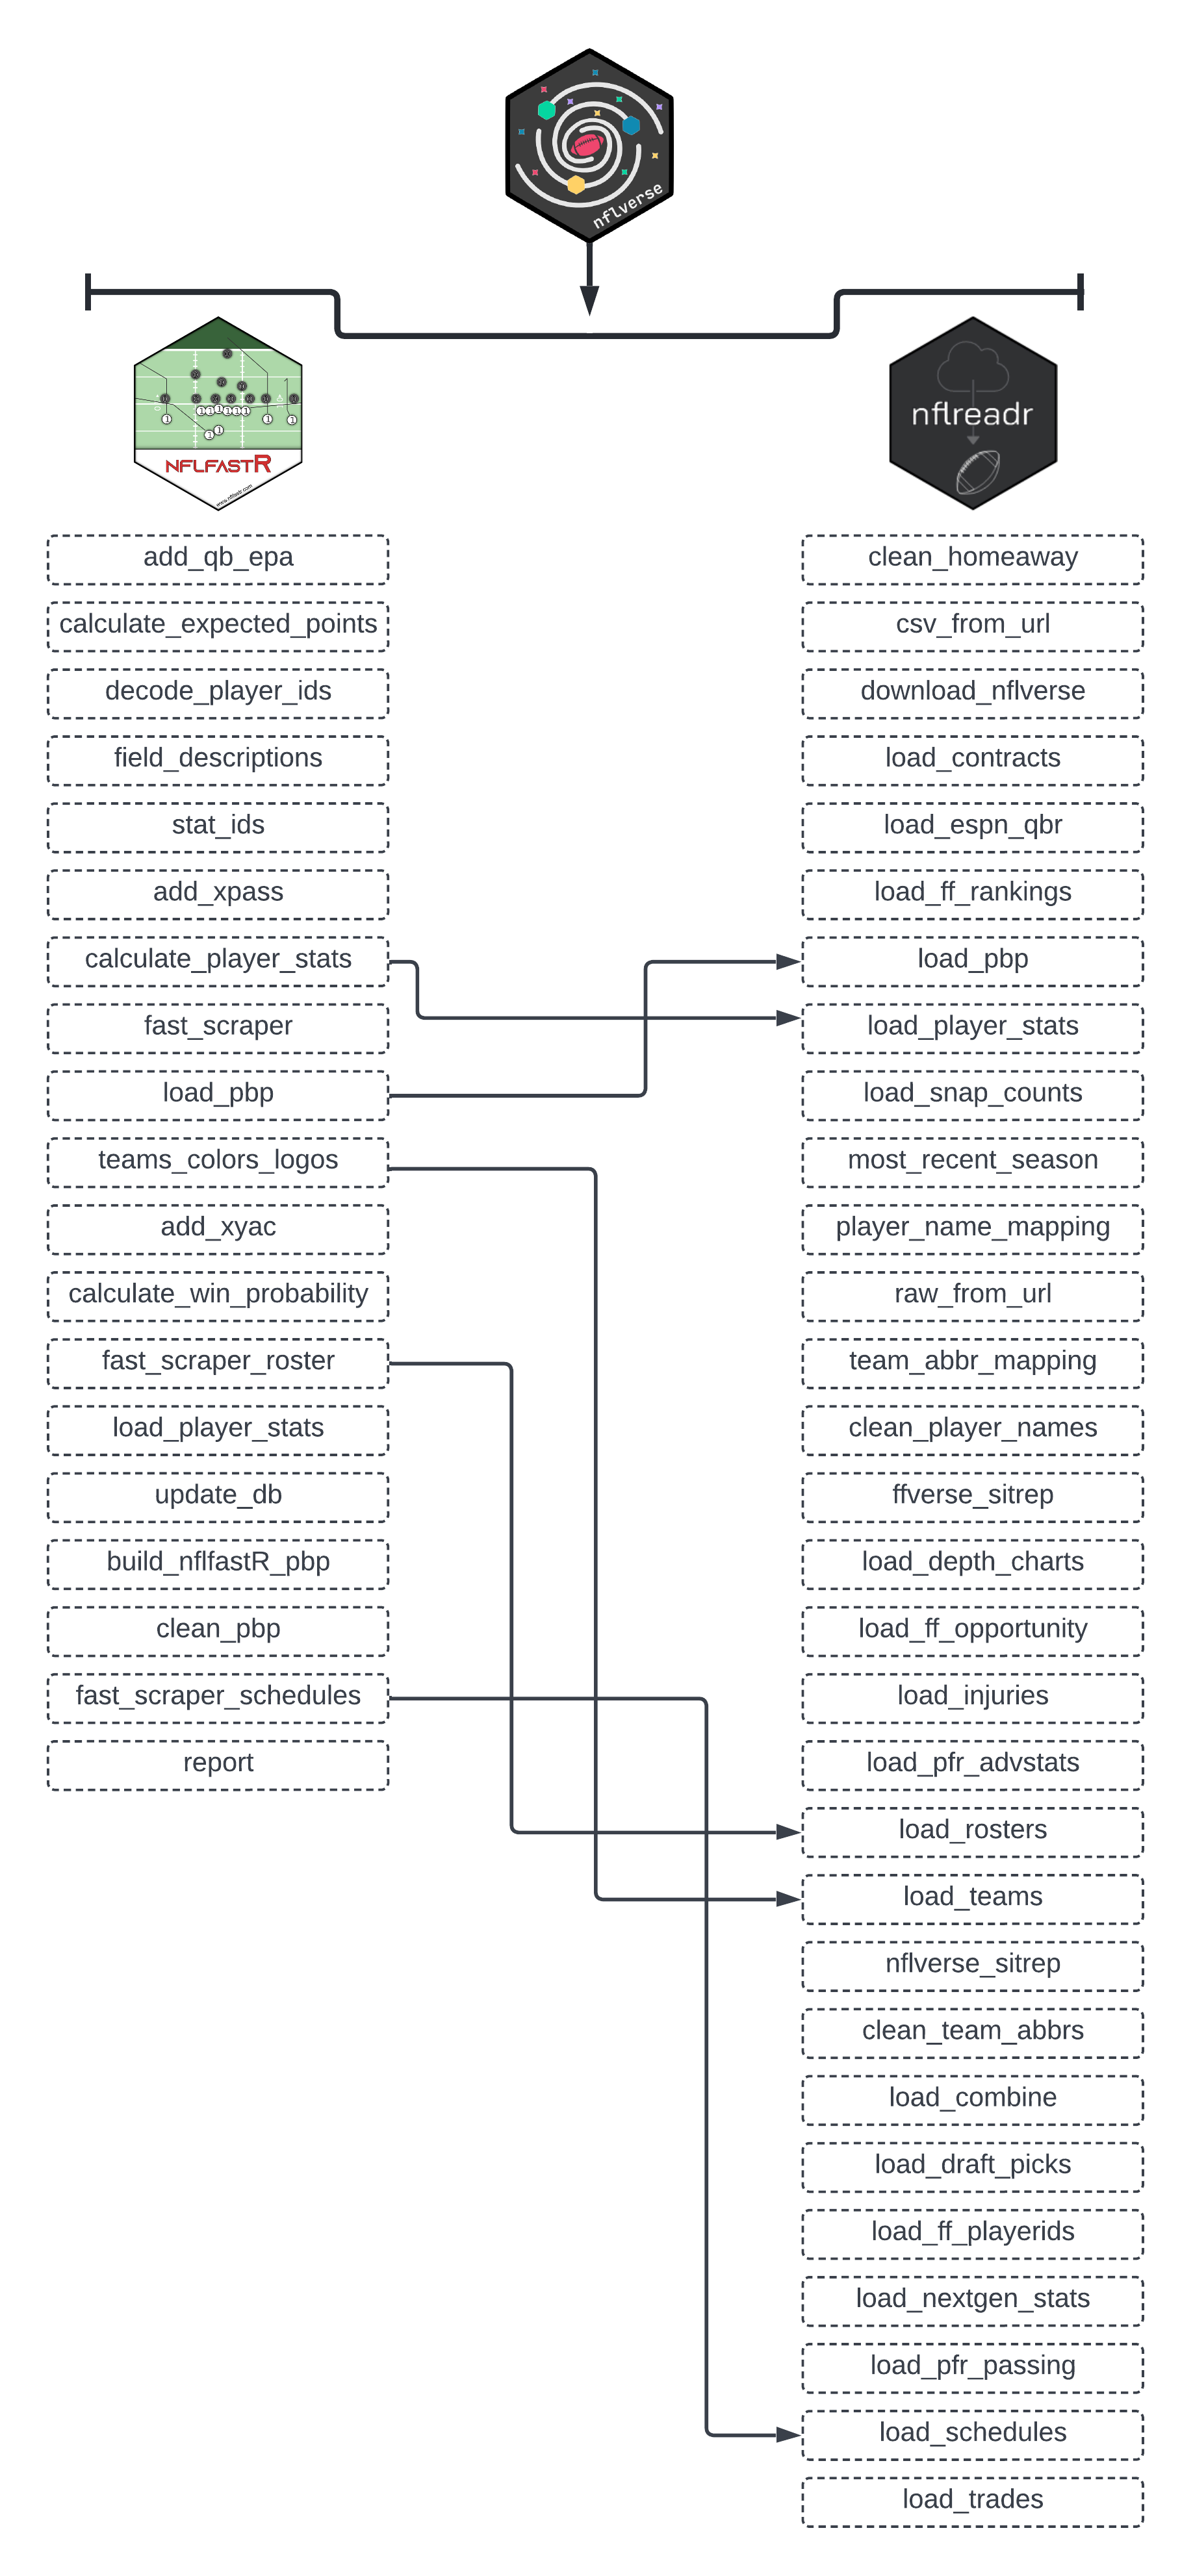
\includegraphics[width=1\textwidth,height=\textheight]{./images/updated-diagram.png}

}

\caption{Comparing nflfastR to nflreadr}

\end{figure}

The purpose of this chapter is to explore \texttt{nflreadr} data in an
introductory fashion using, what I believe, are the two most important
functions in the \texttt{nflverse}: (1.) \texttt{load\_player\_stats()}
and (2.) \texttt{load\_pbp()}. It makes the assumption that you are
versed in the R programming language. If you are not, please start with
Chapter 2 where you can learn about R and the \texttt{tidyverse}
language using examples from the \texttt{nflverse}.

\begin{tcolorbox}[enhanced jigsaw, breakable, leftrule=.75mm, colframe=quarto-callout-important-color-frame, toptitle=1mm, rightrule=.15mm, colbacktitle=quarto-callout-important-color!10!white, colback=white, bottomrule=.15mm, bottomtitle=1mm, titlerule=0mm, coltitle=black, opacitybacktitle=0.6, title=\textcolor{quarto-callout-important-color}{\faExclamation}\hspace{0.5em}{Important}, arc=.35mm, toprule=.15mm, left=2mm, opacityback=0]
If you are completely new to the R programming language (or you have not
yet downloaded and installed both R and RStudio, please read Chapter 2
prior to continuing with this introductory chapter.
\end{tcolorbox}

\hypertarget{nflreadr-an-introduction-to-the-data}{%
\section{\texorpdfstring{\texttt{nflreadr}: An Introduction to the
Data}{nflreadr: An Introduction to the Data}}\label{nflreadr-an-introduction-to-the-data}}

The most important part of the \texttt{nflverse} is, of course, the
data. To begin, we will examine the core data that underpins the
\texttt{nflverse}: weekly player stats and the more detailed
play-by--play data. Using \texttt{nflreadr}, the end user is able to
collect weekly top-level stats via the \texttt{load\_player\_stats()}
function or the much more robust play-by-play numbers by using the
\texttt{load\_pbp()} function.

As you may imagine, there is a \textbf{very important distinction
between the \texttt{load\_player\_stats()}} \textbf{and
\texttt{load\_pbp()}}. As mentioned, \texttt{load\_player\_stats()} will
provide you with weekly, pre-calculated statistics for either offense or
kicking. Conversely, \texttt{load\_pbp()} will provide over 350 metrics
for every single play of every single game dating back to 1999.

The \texttt{load\_player\_stats()} function includes the following
offensive information:

\begin{Shaded}
\begin{Highlighting}[]
\NormalTok{offensive.stats }\OtherTok{\textless{}{-}}\NormalTok{ nflreadr}\SpecialCharTok{::}\FunctionTok{load\_player\_stats}\NormalTok{(}\DecValTok{2021}\NormalTok{)}
\FunctionTok{ls}\NormalTok{(offensive.stats)}
\end{Highlighting}
\end{Shaded}

\begin{verbatim}
 [1] "air_yards_share"             "attempts"                   
 [3] "carries"                     "completions"                
 [5] "dakota"                      "fantasy_points"             
 [7] "fantasy_points_ppr"          "headshot_url"               
 [9] "interceptions"               "pacr"                       
[11] "passing_2pt_conversions"     "passing_air_yards"          
[13] "passing_epa"                 "passing_first_downs"        
[15] "passing_tds"                 "passing_yards"              
[17] "passing_yards_after_catch"   "player_display_name"        
[19] "player_id"                   "player_name"                
[21] "position"                    "position_group"             
[23] "racr"                        "receiving_2pt_conversions"  
[25] "receiving_air_yards"         "receiving_epa"              
[27] "receiving_first_downs"       "receiving_fumbles"          
[29] "receiving_fumbles_lost"      "receiving_tds"              
[31] "receiving_yards"             "receiving_yards_after_catch"
[33] "recent_team"                 "receptions"                 
[35] "rushing_2pt_conversions"     "rushing_epa"                
[37] "rushing_first_downs"         "rushing_fumbles"            
[39] "rushing_fumbles_lost"        "rushing_tds"                
[41] "rushing_yards"               "sack_fumbles"               
[43] "sack_fumbles_lost"           "sack_yards"                 
[45] "sacks"                       "season"                     
[47] "season_type"                 "special_teams_tds"          
[49] "target_share"                "targets"                    
[51] "week"                        "wopr"                       
\end{verbatim}

As well, switching the \texttt{stat\_type} to ``kicking'' provides the
following information:

\begin{Shaded}
\begin{Highlighting}[]
\NormalTok{kicking.stats }\OtherTok{\textless{}{-}}\NormalTok{ nflreadr}\SpecialCharTok{::}\FunctionTok{load\_player\_stats}\NormalTok{(}\DecValTok{2021}\NormalTok{, }\AttributeTok{stat\_type =} \StringTok{"kicking"}\NormalTok{)}
\FunctionTok{ls}\NormalTok{(kicking.stats)}
\end{Highlighting}
\end{Shaded}

\begin{verbatim}
 [1] "fg_att"              "fg_blocked"          "fg_blocked_distance"
 [4] "fg_blocked_list"     "fg_long"             "fg_made"            
 [7] "fg_made_0_19"        "fg_made_20_29"       "fg_made_30_39"      
[10] "fg_made_40_49"       "fg_made_50_59"       "fg_made_60_"        
[13] "fg_made_distance"    "fg_made_list"        "fg_missed"          
[16] "fg_missed_0_19"      "fg_missed_20_29"     "fg_missed_30_39"    
[19] "fg_missed_40_49"     "fg_missed_50_59"     "fg_missed_60_"      
[22] "fg_missed_distance"  "fg_missed_list"      "fg_pct"             
[25] "gwfg_att"            "gwfg_blocked"        "gwfg_distance"      
[28] "gwfg_made"           "gwfg_missed"         "pat_att"            
[31] "pat_blocked"         "pat_made"            "pat_missed"         
[34] "pat_pct"             "player_id"           "player_name"        
[37] "season"              "season_type"         "team"               
[40] "week"               
\end{verbatim}

While the data returned is not as rich as the play-by-play data we will
covering next, the \texttt{load\_player\_stats()} function is extremely
helpful when you need to quickly (and correctly!) recreate the official
stats listed on either the NFL's website or on
\href{https://www.pro-football-reference.com/}{Pro Football Reference}.

As an example, let's say you need to get Ben Roethlisberger's total
passing yard and attempts from the 2021 season. You could do so via
\texttt{load\_pbp()} but, if you do not need further context, using
\texttt{load\_player\_stats()} is much more efficient.

\hypertarget{getting-weekly-player-stats-via-load_player_stats}{%
\subsection{\texorpdfstring{Getting Weekly Player Stats via
\texttt{load\_player\_stats()}}{Getting Weekly Player Stats via load\_player\_stats()}}\label{getting-weekly-player-stats-via-load_player_stats}}

If you are familiar with R, it might seem logical to do the following to
get Roethlisberger's total passing yards and number of attempts from the
2021 regular season:

\begin{Shaded}
\begin{Highlighting}[]
\NormalTok{weekly.data }\OtherTok{\textless{}{-}}\NormalTok{ nflreadr}\SpecialCharTok{::}\FunctionTok{load\_player\_stats}\NormalTok{(}\DecValTok{2021}\NormalTok{)}

\NormalTok{ben.weekly }\OtherTok{\textless{}{-}}\NormalTok{ weekly.data }\SpecialCharTok{\%\textgreater{}\%}
  \FunctionTok{group\_by}\NormalTok{(player\_id, player\_name) }\SpecialCharTok{\%\textgreater{}\%}
  \FunctionTok{filter}\NormalTok{(season\_type }\SpecialCharTok{==} \StringTok{"REG"} \SpecialCharTok{\&}\NormalTok{ player\_name }\SpecialCharTok{==} \StringTok{"B.Roethlisberger"}\NormalTok{) }\SpecialCharTok{\%\textgreater{}\%}
  \FunctionTok{summarize}\NormalTok{(}\AttributeTok{total.yards =} \FunctionTok{sum}\NormalTok{(passing\_yards),}
            \AttributeTok{n.attempts =} \FunctionTok{sum}\NormalTok{(attempts))}
\end{Highlighting}
\end{Shaded}

\begin{verbatim}
`summarise()` has grouped output by 'player_id'. You can override using the
`.groups` argument.
\end{verbatim}

\begin{Shaded}
\begin{Highlighting}[]
\FunctionTok{tibble}\NormalTok{(ben.weekly)}
\end{Highlighting}
\end{Shaded}

\begin{verbatim}
# A tibble: 1 x 4
  player_id  player_name      total.yards n.attempts
  <chr>      <chr>                  <dbl>      <int>
1 00-0022924 B.Roethlisberger        3740        605
\end{verbatim}

As you can see in the \texttt{ben.weekly} output, we have matched his
official 2021 regular stats perfectly with 3,740 passing yards on 605
attempts. The code we just created is doing several things. First, we
are using \texttt{nflreadr::load\_player\_stats(2021)} to place the data
into our R environment in a DF titled \texttt{weekly.data}.

Next, we group the data together by alike \texttt{player\_id} (as every
individual player has a unique ID number) as well as the player's actual
name. At the filtering level, we are looking for just the regular season
(\texttt{REG}) within \texttt{season\_type} and also removing all
quarterbacks except for Ben Roethlisberger. It is important to note that
player names are just first initial and last name, without a space after
the period.

After filtering for the regular season, we are able to summarize all of
the weekly data into combined statistics by summing the weekly totals of
passing yards and attempts.

\textbf{However, filtering by \texttt{player\_name} can lead to
significant issues with your results.} An excellent example of this is
Josh Allen. Let's recreate the code above that successfully provided
Roethlisberger's stats, but replace Ben with Josh Allen:

\begin{Shaded}
\begin{Highlighting}[]
\NormalTok{josh.allen }\OtherTok{\textless{}{-}}\NormalTok{ weekly.data }\SpecialCharTok{\%\textgreater{}\%}
  \FunctionTok{group\_by}\NormalTok{(player\_name) }\SpecialCharTok{\%\textgreater{}\%}
  \FunctionTok{filter}\NormalTok{(player\_name }\SpecialCharTok{==} \StringTok{"J.Allen"} \SpecialCharTok{\&}\NormalTok{ season\_type }\SpecialCharTok{==} \StringTok{"REG"}\NormalTok{) }\SpecialCharTok{\%\textgreater{}\%}
  \FunctionTok{summarize}\NormalTok{(}\AttributeTok{total.yards =} \FunctionTok{sum}\NormalTok{(passing\_yards),}
            \AttributeTok{n.attempts =} \FunctionTok{sum}\NormalTok{(attempts))}

\FunctionTok{tibble}\NormalTok{(josh.allen)}
\end{Highlighting}
\end{Shaded}

\begin{verbatim}
# A tibble: 1 x 3
  player_name total.yards n.attempts
  <chr>             <dbl>      <int>
1 J.Allen            4407        646
\end{verbatim}

The output tells us Allen threw for 4,049 yards on 603 attempts during
the 2021 regular season. A check of his
\href{https://www.pro-football-reference.com/players/A/AlleJo02.htm}{Pro
Football Reference page} tells us those numbers are incorrect. In fact,
he had 4,407 passing yards on 646 attempts. How did we end up 358
passing yards and 43 attempts short?

The answer comes from Aaron Schatz, the creator of
\href{https://www.footballoutsiders.com/}{Football Outsiders}, who
explained in a
\href{https://twitter.com/fo_aschatz/status/1442191416826888192?s=21}{Tweet}
that the official Buffalo Bills' scorer, during week 3 of the NFL
season, decided to refer to Allen as ``Jos.Allen'' as a result of the
Washington Commanders having a player named ``Jonathan Allen.''

To double check this, we can run the same code as above, but remove the
\texttt{player\_name} filter and switch to searching for just those
players on the Buffalo Bills by using \texttt{recent\_team}.

\begin{Shaded}
\begin{Highlighting}[]
\NormalTok{two.josh.allens }\OtherTok{\textless{}{-}}\NormalTok{ weekly.data }\SpecialCharTok{\%\textgreater{}\%}
  \FunctionTok{group\_by}\NormalTok{(player\_id, player\_name) }\SpecialCharTok{\%\textgreater{}\%}
  \FunctionTok{filter}\NormalTok{(season\_type }\SpecialCharTok{==} \StringTok{"REG"} \SpecialCharTok{\&}\NormalTok{ recent\_team }\SpecialCharTok{==} \StringTok{"BUF"}\NormalTok{) }\SpecialCharTok{\%\textgreater{}\%}
  \FunctionTok{summarize}\NormalTok{(}\AttributeTok{total.yards =} \FunctionTok{sum}\NormalTok{(passing\_yards),}
            \AttributeTok{n.attempts =} \FunctionTok{sum}\NormalTok{(attempts))}
\end{Highlighting}
\end{Shaded}

\begin{verbatim}
`summarise()` has grouped output by 'player_id'. You can override using the
`.groups` argument.
\end{verbatim}

\begin{Shaded}
\begin{Highlighting}[]
\FunctionTok{tibble}\NormalTok{(two.josh.allens)}
\end{Highlighting}
\end{Shaded}

\begin{verbatim}
# A tibble: 16 x 4
   player_id  player_name  total.yards n.attempts
   <chr>      <chr>              <dbl>      <int>
 1 00-0027685 E.Sanders              0          0
 2 00-0029000 C.Beasley              0          1
 3 00-0031588 S.Diggs                0          0
 4 00-0031787 J.Kumerow              0          0
 5 00-0033308 M.Breida               0          0
 6 00-0033466 I.McKenzie             0          0
 7 00-0033550 D.Webb                 0          0
 8 00-0033869 M.Trubisky            43          8
 9 00-0033904 D.Dawkins              0          0
10 00-0034857 J.Allen             4407        646
11 00-0035250 D.Singletary           0          0
12 00-0035308 T.Sweeney              0          0
13 00-0035689 D.Knox                 0          0
14 00-0036187 R.Gilliam              0          0
15 00-0036196 G.Davis                0          0
16 00-0036251 Z.Moss                 0          0
\end{verbatim}

Grouping by \texttt{player\_id} and \texttt{player\_name} (as well as
filtering down to Buffalo), we can see that, indeed, Josh Allen is in
the data twice under the same \texttt{player\_id}. Moreover, if you do
the math, you can see that the numbers from his two entries add up to
the official statistics on his Pro Football Reference page.

\hypertarget{using-load_player_stats-correctly}{%
\subsubsection{\texorpdfstring{Using \texttt{load\_player\_stats()}
Correctly}{Using load\_player\_stats() Correctly}}\label{using-load_player_stats-correctly}}

To avoid these situations, you \emph{could} load up NFL rosters via the
\texttt{nflreadr::load\_rosters()} function, but that would require
unnecessary code in order to merge the two DFs together by matching the
\texttt{player\_id} to the \texttt{gsis\_id} number found within the
roster information. Doing so would correct the above issue of Josh Allen
appearing in the data under different spellings. Instead, and to write
the minimal amount of code to complete the task, we can do the
following:

\begin{Shaded}
\begin{Highlighting}[]
\NormalTok{josh.allen }\OtherTok{\textless{}{-}}\NormalTok{ weekly.data }\SpecialCharTok{\%\textgreater{}\%}
  \FunctionTok{filter}\NormalTok{(season\_type }\SpecialCharTok{==} \StringTok{"REG"}\NormalTok{) }\SpecialCharTok{\%\textgreater{}\%}
  \FunctionTok{group\_by}\NormalTok{(player\_id) }\SpecialCharTok{\%\textgreater{}\%}
  \FunctionTok{summarize}\NormalTok{(}\AttributeTok{player\_name =} \FunctionTok{first}\NormalTok{(player\_name),}
            \AttributeTok{total.yards =} \FunctionTok{sum}\NormalTok{(passing\_yards),}
            \AttributeTok{n.attempts =} \FunctionTok{sum}\NormalTok{(attempts)) }\SpecialCharTok{\%\textgreater{}\%}
  \FunctionTok{filter}\NormalTok{(player\_name }\SpecialCharTok{==} \StringTok{"J.Allen"}\NormalTok{)}
\end{Highlighting}
\end{Shaded}

The most efficient way to gather correct player statistics is to do the
\texttt{group\_by} with ONLY the \texttt{player\_id} as, despite the
variation in name, the \texttt{player\_id} remained the same for Josh
Allen. In order to include his correct name in the output, we can gather
QB names within the \texttt{summarize} prior to calculating the sum of
\texttt{passing\_yards} and \texttt{attempts}. After, if you desire to
see only Josh Allen's number, you can filter out to just his name.

\hypertarget{using-load_player_stats-to-find-leaders}{%
\subsection{\texorpdfstring{Using \texttt{load\_player\_stats()} To Find
Leaders}{Using load\_player\_stats() To Find Leaders}}\label{using-load_player_stats-to-find-leaders}}

While using \texttt{load\_player\_stats()} does not provide the ability
to add context to your analysis as we will soon see with
\texttt{load\_pbp()}, it does provide an easy and efficient way to
determine weekly or season-long leaders over many top-level, widely-used
NFL statistics. In the below example, we will determine the 2021 leaders
in air yards per attempt.

\hypertarget{an-example-2021-qb-air-yards-per-attempt-leaders}{%
\subsubsection{An Example: 2021 QB Air Yards per Attempt
Leaders}\label{an-example-2021-qb-air-yards-per-attempt-leaders}}

\begin{Shaded}
\begin{Highlighting}[]
\NormalTok{data }\OtherTok{\textless{}{-}}\NormalTok{ nflreadr}\SpecialCharTok{::}\FunctionTok{load\_player\_stats}\NormalTok{(}\DecValTok{2021}\NormalTok{)}

\NormalTok{ay.per.attempt }\OtherTok{\textless{}{-}}\NormalTok{ data }\SpecialCharTok{\%\textgreater{}\%}
  \FunctionTok{group\_by}\NormalTok{(player\_id) }\SpecialCharTok{\%\textgreater{}\%}
  \FunctionTok{filter}\NormalTok{(season\_type }\SpecialCharTok{==} \StringTok{"REG"}\NormalTok{) }\SpecialCharTok{\%\textgreater{}\%}
  \FunctionTok{summarize}\NormalTok{(}\AttributeTok{player\_name =} \FunctionTok{first}\NormalTok{(player\_name),}
            \AttributeTok{n.attempts =} \FunctionTok{sum}\NormalTok{(attempts),}
            \AttributeTok{n.airyards =} \FunctionTok{sum}\NormalTok{(passing\_air\_yards),}
            \AttributeTok{ay.attempt =}\NormalTok{ n.airyards }\SpecialCharTok{/}\NormalTok{ n.attempts) }\SpecialCharTok{\%\textgreater{}\%}
  \FunctionTok{filter}\NormalTok{(n.attempts }\SpecialCharTok{\textgreater{}=} \DecValTok{400}\NormalTok{) }\SpecialCharTok{\%\textgreater{}\%}
  \FunctionTok{select}\NormalTok{(player\_name, ay.attempt) }\SpecialCharTok{\%\textgreater{}\%}
  \FunctionTok{arrange}\NormalTok{(}\SpecialCharTok{{-}}\NormalTok{ay.attempt)}
\end{Highlighting}
\end{Shaded}

In the above example, we are using \texttt{group\_by} to combine the
desired statistics based on each unique \texttt{player\_id} to, again,
avoid any issues with player names within the data. After filtering to
include just those statistics for the regular season, we first use the
\texttt{summarize} function to grab the first \texttt{player\_name}
associated with the \texttt{player\_id}. After, we find two items: (1.)
the total number of passing attempts by each QB which is outputted into
a new row titled \texttt{n.attempts} and the regular season total of
each QB's air yards, again outputted into a new row titled
\texttt{n.airyards}.

It is important to note that the final row created with the
\texttt{summarize} function is not a statistic included within
\texttt{load\_player\_stats()}. In order to find a QB's average air
yards per attempt, we must use the first two items we've created and do
some simple division (the created \texttt{n.airyards} divided by
\texttt{n.attempts}).

Finally, to ``clear the noise'' of those QBs with minimal attempts
through the season, we included a filter to include only those passers
with at least 400 attempts. After, we arrange the new DF by sorting the
QBs in descending order by average air yards per attempt.

The end results look like this:

\begin{Shaded}
\begin{Highlighting}[]
\FunctionTok{tibble}\NormalTok{(ay.per.attempt)}
\end{Highlighting}
\end{Shaded}

\begin{verbatim}
# A tibble: 25 x 2
   player_name   ay.attempt
   <chr>              <dbl>
 1 R.Wilson            9.89
 2 J.Hurts             8.99
 3 B.Mayfield          8.73
 4 M.Stafford          8.48
 5 J.Allen             8.20
 6 K.Cousins           8.16
 7 J.Burrow            8.12
 8 D.Carr              8.12
 9 T.Brady             8.10
10 T.Bridgewater       8.04
# ... with 15 more rows
\end{verbatim}

Russell Wilson led the NFL in 2021 with 9.89 air yards per attempt.

\hypertarget{using-load_pbp-to-add-context-to-statistics}{%
\section{\texorpdfstring{Using \texttt{load\_pbp()} to Add Context to
Statistics}{Using load\_pbp() to Add Context to Statistics}}\label{using-load_pbp-to-add-context-to-statistics}}

As just mentioned above, using the \texttt{load\_pbp()} function is
preferable when you are looking to add context to a player's statistics,
as the \texttt{load\_player\_stats()} function is, for all intents and
purposes, aggregated statistics that limit your ability to find deeper
meaning.

The \texttt{load\_pbp()} function provides over 350 various metrics, as
listed below:

\begin{Shaded}
\begin{Highlighting}[]
\NormalTok{pbp.data }\OtherTok{\textless{}{-}}\NormalTok{ nflreadr}\SpecialCharTok{::}\FunctionTok{load\_pbp}\NormalTok{(}\DecValTok{2021}\NormalTok{)}
\FunctionTok{ls}\NormalTok{(pbp.data)}
\end{Highlighting}
\end{Shaded}

\begin{verbatim}
  [1] "aborted_play"                        
  [2] "air_epa"                             
  [3] "air_wpa"                             
  [4] "air_yards"                           
  [5] "assist_tackle"                       
  [6] "assist_tackle_1_player_id"           
  [7] "assist_tackle_1_player_name"         
  [8] "assist_tackle_1_team"                
  [9] "assist_tackle_2_player_id"           
 [10] "assist_tackle_2_player_name"         
 [11] "assist_tackle_2_team"                
 [12] "assist_tackle_3_player_id"           
 [13] "assist_tackle_3_player_name"         
 [14] "assist_tackle_3_team"                
 [15] "assist_tackle_4_player_id"           
 [16] "assist_tackle_4_player_name"         
 [17] "assist_tackle_4_team"                
 [18] "away_coach"                          
 [19] "away_score"                          
 [20] "away_team"                           
 [21] "away_timeouts_remaining"             
 [22] "away_wp"                             
 [23] "away_wp_post"                        
 [24] "blocked_player_id"                   
 [25] "blocked_player_name"                 
 [26] "comp_air_epa"                        
 [27] "comp_air_wpa"                        
 [28] "comp_yac_epa"                        
 [29] "comp_yac_wpa"                        
 [30] "complete_pass"                       
 [31] "cp"                                  
 [32] "cpoe"                                
 [33] "def_wp"                              
 [34] "defensive_extra_point_attempt"       
 [35] "defensive_extra_point_conv"          
 [36] "defensive_two_point_attempt"         
 [37] "defensive_two_point_conv"            
 [38] "defteam"                             
 [39] "defteam_score"                       
 [40] "defteam_score_post"                  
 [41] "defteam_timeouts_remaining"          
 [42] "desc"                                
 [43] "div_game"                            
 [44] "down"                                
 [45] "drive"                               
 [46] "drive_end_transition"                
 [47] "drive_end_yard_line"                 
 [48] "drive_ended_with_score"              
 [49] "drive_first_downs"                   
 [50] "drive_game_clock_end"                
 [51] "drive_game_clock_start"              
 [52] "drive_inside20"                      
 [53] "drive_play_count"                    
 [54] "drive_play_id_ended"                 
 [55] "drive_play_id_started"               
 [56] "drive_quarter_end"                   
 [57] "drive_quarter_start"                 
 [58] "drive_real_start_time"               
 [59] "drive_start_transition"              
 [60] "drive_start_yard_line"               
 [61] "drive_time_of_possession"            
 [62] "drive_yards_penalized"               
 [63] "end_clock_time"                      
 [64] "end_yard_line"                       
 [65] "ep"                                  
 [66] "epa"                                 
 [67] "extra_point_attempt"                 
 [68] "extra_point_prob"                    
 [69] "extra_point_result"                  
 [70] "fantasy"                             
 [71] "fantasy_id"                          
 [72] "fantasy_player_id"                   
 [73] "fantasy_player_name"                 
 [74] "fg_prob"                             
 [75] "field_goal_attempt"                  
 [76] "field_goal_result"                   
 [77] "first_down"                          
 [78] "first_down_pass"                     
 [79] "first_down_penalty"                  
 [80] "first_down_rush"                     
 [81] "fixed_drive"                         
 [82] "fixed_drive_result"                  
 [83] "forced_fumble_player_1_player_id"    
 [84] "forced_fumble_player_1_player_name"  
 [85] "forced_fumble_player_1_team"         
 [86] "forced_fumble_player_2_player_id"    
 [87] "forced_fumble_player_2_player_name"  
 [88] "forced_fumble_player_2_team"         
 [89] "fourth_down_converted"               
 [90] "fourth_down_failed"                  
 [91] "fumble"                              
 [92] "fumble_forced"                       
 [93] "fumble_lost"                         
 [94] "fumble_not_forced"                   
 [95] "fumble_out_of_bounds"                
 [96] "fumble_recovery_1_player_id"         
 [97] "fumble_recovery_1_player_name"       
 [98] "fumble_recovery_1_team"              
 [99] "fumble_recovery_1_yards"             
[100] "fumble_recovery_2_player_id"         
[101] "fumble_recovery_2_player_name"       
[102] "fumble_recovery_2_team"              
[103] "fumble_recovery_2_yards"             
[104] "fumbled_1_player_id"                 
[105] "fumbled_1_player_name"               
[106] "fumbled_1_team"                      
[107] "fumbled_2_player_id"                 
[108] "fumbled_2_player_name"               
[109] "fumbled_2_team"                      
[110] "game_date"                           
[111] "game_half"                           
[112] "game_id"                             
[113] "game_seconds_remaining"              
[114] "game_stadium"                        
[115] "goal_to_go"                          
[116] "half_sack_1_player_id"               
[117] "half_sack_1_player_name"             
[118] "half_sack_2_player_id"               
[119] "half_sack_2_player_name"             
[120] "half_seconds_remaining"              
[121] "home_coach"                          
[122] "home_opening_kickoff"                
[123] "home_score"                          
[124] "home_team"                           
[125] "home_timeouts_remaining"             
[126] "home_wp"                             
[127] "home_wp_post"                        
[128] "id"                                  
[129] "incomplete_pass"                     
[130] "interception"                        
[131] "interception_player_id"              
[132] "interception_player_name"            
[133] "jersey_number"                       
[134] "kick_distance"                       
[135] "kicker_player_id"                    
[136] "kicker_player_name"                  
[137] "kickoff_attempt"                     
[138] "kickoff_downed"                      
[139] "kickoff_fair_catch"                  
[140] "kickoff_in_endzone"                  
[141] "kickoff_inside_twenty"               
[142] "kickoff_out_of_bounds"               
[143] "kickoff_returner_player_id"          
[144] "kickoff_returner_player_name"        
[145] "lateral_interception_player_id"      
[146] "lateral_interception_player_name"    
[147] "lateral_kickoff_returner_player_id"  
[148] "lateral_kickoff_returner_player_name"
[149] "lateral_punt_returner_player_id"     
[150] "lateral_punt_returner_player_name"   
[151] "lateral_receiver_player_id"          
[152] "lateral_receiver_player_name"        
[153] "lateral_receiving_yards"             
[154] "lateral_reception"                   
[155] "lateral_recovery"                    
[156] "lateral_return"                      
[157] "lateral_rush"                        
[158] "lateral_rusher_player_id"            
[159] "lateral_rusher_player_name"          
[160] "lateral_rushing_yards"               
[161] "lateral_sack_player_id"              
[162] "lateral_sack_player_name"            
[163] "location"                            
[164] "name"                                
[165] "nfl_api_id"                          
[166] "no_huddle"                           
[167] "no_score_prob"                       
[168] "old_game_id"                         
[169] "opp_fg_prob"                         
[170] "opp_safety_prob"                     
[171] "opp_td_prob"                         
[172] "order_sequence"                      
[173] "out_of_bounds"                       
[174] "own_kickoff_recovery"                
[175] "own_kickoff_recovery_player_id"      
[176] "own_kickoff_recovery_player_name"    
[177] "own_kickoff_recovery_td"             
[178] "pass"                                
[179] "pass_attempt"                        
[180] "pass_defense_1_player_id"            
[181] "pass_defense_1_player_name"          
[182] "pass_defense_2_player_id"            
[183] "pass_defense_2_player_name"          
[184] "pass_length"                         
[185] "pass_location"                       
[186] "pass_oe"                             
[187] "pass_touchdown"                      
[188] "passer"                              
[189] "passer_id"                           
[190] "passer_jersey_number"                
[191] "passer_player_id"                    
[192] "passer_player_name"                  
[193] "passing_yards"                       
[194] "penalty"                             
[195] "penalty_player_id"                   
[196] "penalty_player_name"                 
[197] "penalty_team"                        
[198] "penalty_type"                        
[199] "penalty_yards"                       
[200] "play"                                
[201] "play_clock"                          
[202] "play_deleted"                        
[203] "play_id"                             
[204] "play_type"                           
[205] "play_type_nfl"                       
[206] "posteam"                             
[207] "posteam_score"                       
[208] "posteam_score_post"                  
[209] "posteam_timeouts_remaining"          
[210] "posteam_type"                        
[211] "punt_attempt"                        
[212] "punt_blocked"                        
[213] "punt_downed"                         
[214] "punt_fair_catch"                     
[215] "punt_in_endzone"                     
[216] "punt_inside_twenty"                  
[217] "punt_out_of_bounds"                  
[218] "punt_returner_player_id"             
[219] "punt_returner_player_name"           
[220] "punter_player_id"                    
[221] "punter_player_name"                  
[222] "qb_dropback"                         
[223] "qb_epa"                              
[224] "qb_hit"                              
[225] "qb_hit_1_player_id"                  
[226] "qb_hit_1_player_name"                
[227] "qb_hit_2_player_id"                  
[228] "qb_hit_2_player_name"                
[229] "qb_kneel"                            
[230] "qb_scramble"                         
[231] "qb_spike"                            
[232] "qtr"                                 
[233] "quarter_end"                         
[234] "quarter_seconds_remaining"           
[235] "receiver"                            
[236] "receiver_id"                         
[237] "receiver_jersey_number"              
[238] "receiver_player_id"                  
[239] "receiver_player_name"                
[240] "receiving_yards"                     
[241] "replay_or_challenge"                 
[242] "replay_or_challenge_result"          
[243] "result"                              
[244] "return_team"                         
[245] "return_touchdown"                    
[246] "return_yards"                        
[247] "roof"                                
[248] "run_gap"                             
[249] "run_location"                        
[250] "rush"                                
[251] "rush_attempt"                        
[252] "rush_touchdown"                      
[253] "rusher"                              
[254] "rusher_id"                           
[255] "rusher_jersey_number"                
[256] "rusher_player_id"                    
[257] "rusher_player_name"                  
[258] "rushing_yards"                       
[259] "sack"                                
[260] "sack_player_id"                      
[261] "sack_player_name"                    
[262] "safety"                              
[263] "safety_player_id"                    
[264] "safety_player_name"                  
[265] "safety_prob"                         
[266] "score_differential"                  
[267] "score_differential_post"             
[268] "season"                              
[269] "season_type"                         
[270] "series"                              
[271] "series_result"                       
[272] "series_success"                      
[273] "shotgun"                             
[274] "side_of_field"                       
[275] "solo_tackle"                         
[276] "solo_tackle_1_player_id"             
[277] "solo_tackle_1_player_name"           
[278] "solo_tackle_1_team"                  
[279] "solo_tackle_2_player_id"             
[280] "solo_tackle_2_player_name"           
[281] "solo_tackle_2_team"                  
[282] "sp"                                  
[283] "special"                             
[284] "special_teams_play"                  
[285] "spread_line"                         
[286] "st_play_type"                        
[287] "stadium"                             
[288] "stadium_id"                          
[289] "start_time"                          
[290] "success"                             
[291] "surface"                             
[292] "tackle_for_loss_1_player_id"         
[293] "tackle_for_loss_1_player_name"       
[294] "tackle_for_loss_2_player_id"         
[295] "tackle_for_loss_2_player_name"       
[296] "tackle_with_assist"                  
[297] "tackle_with_assist_1_player_id"      
[298] "tackle_with_assist_1_player_name"    
[299] "tackle_with_assist_1_team"           
[300] "tackle_with_assist_2_player_id"      
[301] "tackle_with_assist_2_player_name"    
[302] "tackle_with_assist_2_team"           
[303] "tackled_for_loss"                    
[304] "td_player_id"                        
[305] "td_player_name"                      
[306] "td_prob"                             
[307] "td_team"                             
[308] "temp"                                
[309] "third_down_converted"                
[310] "third_down_failed"                   
[311] "time"                                
[312] "time_of_day"                         
[313] "timeout"                             
[314] "timeout_team"                        
[315] "total"                               
[316] "total_away_comp_air_epa"             
[317] "total_away_comp_air_wpa"             
[318] "total_away_comp_yac_epa"             
[319] "total_away_comp_yac_wpa"             
[320] "total_away_epa"                      
[321] "total_away_pass_epa"                 
[322] "total_away_pass_wpa"                 
[323] "total_away_raw_air_epa"              
[324] "total_away_raw_air_wpa"              
[325] "total_away_raw_yac_epa"              
[326] "total_away_raw_yac_wpa"              
[327] "total_away_rush_epa"                 
[328] "total_away_rush_wpa"                 
[329] "total_away_score"                    
[330] "total_home_comp_air_epa"             
[331] "total_home_comp_air_wpa"             
[332] "total_home_comp_yac_epa"             
[333] "total_home_comp_yac_wpa"             
[334] "total_home_epa"                      
[335] "total_home_pass_epa"                 
[336] "total_home_pass_wpa"                 
[337] "total_home_raw_air_epa"              
[338] "total_home_raw_air_wpa"              
[339] "total_home_raw_yac_epa"              
[340] "total_home_raw_yac_wpa"              
[341] "total_home_rush_epa"                 
[342] "total_home_rush_wpa"                 
[343] "total_home_score"                    
[344] "total_line"                          
[345] "touchback"                           
[346] "touchdown"                           
[347] "two_point_attempt"                   
[348] "two_point_conv_result"               
[349] "two_point_conversion_prob"           
[350] "vegas_home_wp"                       
[351] "vegas_home_wpa"                      
[352] "vegas_wp"                            
[353] "vegas_wpa"                           
[354] "weather"                             
[355] "week"                                
[356] "wind"                                
[357] "wp"                                  
[358] "wpa"                                 
[359] "xpass"                               
[360] "xyac_epa"                            
[361] "xyac_fd"                             
[362] "xyac_mean_yardage"                   
[363] "xyac_median_yardage"                 
[364] "xyac_success"                        
[365] "yac_epa"                             
[366] "yac_wpa"                             
[367] "yardline_100"                        
[368] "yards_after_catch"                   
[369] "yards_gained"                        
[370] "ydsnet"                              
[371] "ydstogo"                             
[372] "yrdln"                               
\end{verbatim}

A bit overwhelming, right?

Luckily, the \texttt{nflfastR} website includes a searchable directory
of all the variables with a brief description of what each one means.
You can visit that here:
\href{https://www.nflfastr.com/articles/field_descriptions.html}{nflfastR
Field Descriptions}.

As seen above, we can use the \texttt{load\_player\_stats()} function to
determine a QB's average yards per attempt over the course of a season.
But, what if we wanted to add context to that? For example, how do we
explore a QB's air yards in game-specific situations?

To showcase using \texttt{load\_pbp()} to add context to your analysis,
let's explore QB performance via air yards on 3rd down.

\hypertarget{an-example-qb-aggressiveness-on-3rd-down}{%
\subsection{An Example: QB Aggressiveness on 3rd
Down}\label{an-example-qb-aggressiveness-on-3rd-down}}

Sticking with the air yards example from above, let's examine a metric I
created using \texttt{load\_pbp()} that I coined \textbf{QB 3rd Down
Aggressiveness}. The metric is designed to determine which QBs in the
NFL are most aggressive in 3rd down situations by gauging how often they
throw the ball to, or pass, the first down line. It is an interesting
metric to explore as, just like many metrics in the NFL, not all air
yards are created equal. For example, eight air yards on 1st and 10 are
less valuable than the same eight air yards on 3rd and 5.

First, let's highlight the code used to create the results for this
metric and then break it down line-by-line.

\begin{Shaded}
\begin{Highlighting}[]
\NormalTok{data }\OtherTok{\textless{}{-}}\NormalTok{ nflreadr}\SpecialCharTok{::}\FunctionTok{load\_pbp}\NormalTok{(}\DecValTok{2021}\NormalTok{)}

\NormalTok{aggressiveness }\OtherTok{\textless{}{-}}\NormalTok{ data }\SpecialCharTok{\%\textgreater{}\%}
  \FunctionTok{group\_by}\NormalTok{(passer\_id) }\SpecialCharTok{\%\textgreater{}\%}
  \FunctionTok{filter}\NormalTok{(down }\SpecialCharTok{==} \DecValTok{3}\NormalTok{, play\_type }\SpecialCharTok{==} \StringTok{"pass"}\NormalTok{, ydstogo }\SpecialCharTok{\textgreater{}=} \DecValTok{5}\NormalTok{, ydstogo }\SpecialCharTok{\textless{}=} \DecValTok{10}\NormalTok{) }\SpecialCharTok{\%\textgreater{}\%}
  \FunctionTok{summarize}\NormalTok{(}\AttributeTok{player\_name =} \FunctionTok{first}\NormalTok{(passer),}
            \AttributeTok{team =} \FunctionTok{first}\NormalTok{(posteam),}
            \AttributeTok{total =} \FunctionTok{n}\NormalTok{(),}
            \AttributeTok{aggressive =} \FunctionTok{sum}\NormalTok{(air\_yards }\SpecialCharTok{\textgreater{}=}\NormalTok{ ydstogo, }\AttributeTok{na.rm =} \ConstantTok{TRUE}\NormalTok{),}
            \AttributeTok{percentage =}\NormalTok{ aggressive }\SpecialCharTok{/}\NormalTok{ total) }\SpecialCharTok{\%\textgreater{}\%}
  \FunctionTok{filter}\NormalTok{(total }\SpecialCharTok{\textgreater{}=} \DecValTok{50}\NormalTok{) }\SpecialCharTok{\%\textgreater{}\%}
  \FunctionTok{arrange}\NormalTok{(}\SpecialCharTok{{-}}\NormalTok{percentage)}

\FunctionTok{tibble}\NormalTok{(aggressiveness)}
\end{Highlighting}
\end{Shaded}

\begin{verbatim}
# A tibble: 30 x 6
   passer_id  player_name  team  total aggressive percentage
   <chr>      <chr>        <chr> <int>      <int>      <dbl>
 1 00-0033077 D.Prescott   DAL      84         53      0.631
 2 00-0035228 K.Murray     ARI      60         37      0.617
 3 00-0036389 J.Hurts      PHI      65         40      0.615
 4 00-0033873 P.Mahomes    KC       93         56      0.602
 5 00-0034855 B.Mayfield   CLE      59         35      0.593
 6 00-0036971 T.Lawrence   JAX      78         46      0.590
 7 00-0036355 J.Herbert    LAC      87         51      0.586
 8 00-0035710 D.Jones      NYG      60         35      0.583
 9 00-0036212 T.Tagovailoa MIA      60         35      0.583
10 00-0026498 M.Stafford   LA       95         54      0.568
# ... with 20 more rows
\end{verbatim}

As you can see in the \texttt{tibble()} output of the results, Dak
Prescott was the most aggressive quarterback in 3rd down passing
situations in the 2021 season, passing to, our beyond, the line of gain
just over 63\% of the time.

After creating a new dataframe called \texttt{aggressiveness} from the
2021 play-by-play we originally collected using
\texttt{data\ \textless{}-\ nflreadr::load\_pbp(2021)}, we use
\texttt{group\_by} to ensure that the data is being collected \emph{per
individual quarterback} via \texttt{passer\_id.}

After using the \texttt{group\_by} function to lump data with each
individual QB, we then use \texttt{filter()} function. Of course, we
only want those \texttt{play\_types} that are ``pass'' on 3rd downs.
However, in the above code, we are filtering for \emph{just}~those 3rd
down situations where the \texttt{yards\ to\ go} are between five and
ten yards.

Doing so was a personal decision on my end when creating the metric, as
there are certainly arguments to be made regarding how to ``capture''
scenarios in the data that require ``aggressiveness.'' My logic? If
there were less than five yards to go on 3rd down, the opposing defense
would not be able to ``sell out'' to the pass as it would not be out of
the question for an offense to attempt to gain the first down on the
ground. Conversely, anything \emph{over} ten yards likely results in the
defense selling out to the pass, thus leaving an imprint on the
aggressiveness output of the quarterbacks.

For the sake of curiosity, we can edit the above code to include all
passing attempts on 3rd down with under 10 yards to go for the first
down:

\begin{Shaded}
\begin{Highlighting}[]
\NormalTok{aggressiveness.under}\FloatTok{.10} \OtherTok{\textless{}{-}}\NormalTok{ data }\SpecialCharTok{\%\textgreater{}\%}
  \FunctionTok{group\_by}\NormalTok{(passer\_id) }\SpecialCharTok{\%\textgreater{}\%}
  \FunctionTok{filter}\NormalTok{(down }\SpecialCharTok{==} \DecValTok{3}\NormalTok{, play\_type }\SpecialCharTok{==} \StringTok{"pass"}\NormalTok{, ydstogo }\SpecialCharTok{\textless{}=} \DecValTok{10}\NormalTok{) }\SpecialCharTok{\%\textgreater{}\%}
  \FunctionTok{summarize}\NormalTok{(}\AttributeTok{player\_name =} \FunctionTok{first}\NormalTok{(passer),}
            \AttributeTok{team =} \FunctionTok{first}\NormalTok{(posteam),}
            \AttributeTok{total =} \FunctionTok{n}\NormalTok{(),}
            \AttributeTok{aggressive =} \FunctionTok{sum}\NormalTok{(air\_yards }\SpecialCharTok{\textgreater{}=}\NormalTok{ ydstogo, }\AttributeTok{na.rm =} \ConstantTok{TRUE}\NormalTok{),}
            \AttributeTok{percentage =}\NormalTok{ aggressive }\SpecialCharTok{/}\NormalTok{ total) }\SpecialCharTok{\%\textgreater{}\%}
  \FunctionTok{filter}\NormalTok{(total }\SpecialCharTok{\textgreater{}=} \DecValTok{50}\NormalTok{) }\SpecialCharTok{\%\textgreater{}\%}
  \FunctionTok{arrange}\NormalTok{(}\FunctionTok{desc}\NormalTok{(percentage))}

\FunctionTok{tibble}\NormalTok{(aggressiveness.under}\FloatTok{.10}\NormalTok{)}
\end{Highlighting}
\end{Shaded}

\begin{verbatim}
# A tibble: 33 x 6
   passer_id  player_name  team  total aggressive percentage
   <chr>      <chr>        <chr> <int>      <int>      <dbl>
 1 00-0035228 K.Murray     ARI      98         67      0.684
 2 00-0036389 J.Hurts      PHI     107         73      0.682
 3 00-0036971 T.Lawrence   JAX     131         88      0.672
 4 00-0033077 D.Prescott   DAL     136         89      0.654
 5 00-0034857 J.Allen      BUF     138         88      0.638
 6 00-0036355 J.Herbert    LAC     148         94      0.635
 7 00-0036212 T.Tagovailoa MIA      93         59      0.634
 8 00-0026498 M.Stafford   LA      172        109      0.634
 9 00-0023459 A.Rodgers    GB      128         80      0.625
10 00-0035710 D.Jones      NYG      85         53      0.624
# ... with 23 more rows
\end{verbatim}

The results are quite different from the first running of this metric,
as Dak Prescott is now the 4th most aggressive QB, while Kyler Murray
moves to the top by approaching a nearly 70\% aggressiveness rate on 3rd
down. This small change highlights an important element about analytics:
much of the work is the result of the coder (ie., \uline{you}) being
able to justify your decision-making process when developing the filters
for each metric you create.

In this case, I stand by my argument that including just those pass
attempts on 3rd down with between 5 and 10 yards to go is a more
accurate assessment of aggressiveness as, for example, 3rd down with 8
yards to go is an obvious passing situation in \uline{most} cases.

That begs the question, though: in which cases is 3rd down with 8 yards
to go \uline{not} an obvious passing situation? An example of this falls
under the guise of ``garbage time.''

\hypertarget{qb-aggressiveness-filtering-for-garbage-time}{%
\subsubsection{QB Aggressiveness: Filtering for ``Garbage
Time?''}\label{qb-aggressiveness-filtering-for-garbage-time}}

In our initial running of the QB Aggressiveness metric, Josh Allen is
the 15th most aggressive QB in the NFL on 3rd down with between 5 and 10
yards to go. But how much does the success of the Buffalo Bills play
into that 15th place ranking?

The Bills, at the conclusion of the 2021 season, had the largest
positive point differential in the league at 194 (the Bills scored 483
points, while allowing just 289). Perhaps Allen's numbers are skewed
because the Bills were so often playing with the lead late into the
game?

To account for this, we can add information into the \texttt{filter()}
function to attempt to remove what are referenced to in the analytics
community as ``garbage time stats.''

Let's add the ``garbage time'' filter to the code we've already
prepared:

\begin{Shaded}
\begin{Highlighting}[]
\NormalTok{aggressiveness.garbage }\OtherTok{\textless{}{-}}\NormalTok{ data }\SpecialCharTok{\%\textgreater{}\%}
  \FunctionTok{group\_by}\NormalTok{(passer\_id) }\SpecialCharTok{\%\textgreater{}\%}
  \FunctionTok{filter}\NormalTok{(down }\SpecialCharTok{==} \DecValTok{3}\NormalTok{, play\_type }\SpecialCharTok{==} \StringTok{"pass"}\NormalTok{, ydstogo }\SpecialCharTok{\textgreater{}=} \DecValTok{5}\NormalTok{, ydstogo }\SpecialCharTok{\textless{}=} \DecValTok{10}\NormalTok{,}
\NormalTok{         wp }\SpecialCharTok{\textgreater{}}\NormalTok{ .}\DecValTok{05}\NormalTok{, wp }\SpecialCharTok{\textless{}}\NormalTok{ .}\DecValTok{95}\NormalTok{, half\_seconds\_remaining }\SpecialCharTok{\textgreater{}} \DecValTok{120}\NormalTok{) }\SpecialCharTok{\%\textgreater{}\%}
  \FunctionTok{summarize}\NormalTok{(}\AttributeTok{player\_name =} \FunctionTok{first}\NormalTok{(passer),}
            \AttributeTok{team =} \FunctionTok{first}\NormalTok{(posteam),}
            \AttributeTok{total =} \FunctionTok{n}\NormalTok{(),}
            \AttributeTok{aggressive =} \FunctionTok{sum}\NormalTok{(air\_yards }\SpecialCharTok{\textgreater{}=}\NormalTok{ ydstogo, }\AttributeTok{na.rm =} \ConstantTok{TRUE}\NormalTok{),}
            \AttributeTok{percentage =}\NormalTok{ aggressive }\SpecialCharTok{/}\NormalTok{ total) }\SpecialCharTok{\%\textgreater{}\%}
  \FunctionTok{filter}\NormalTok{(total }\SpecialCharTok{\textgreater{}=} \DecValTok{50}\NormalTok{) }\SpecialCharTok{\%\textgreater{}\%}
  \FunctionTok{arrange}\NormalTok{(}\FunctionTok{desc}\NormalTok{(percentage))}

\FunctionTok{tibble}\NormalTok{(aggressiveness.garbage)}
\end{Highlighting}
\end{Shaded}

\begin{verbatim}
# A tibble: 26 x 6
   passer_id  player_name team  total aggressive percentage
   <chr>      <chr>       <chr> <int>      <int>      <dbl>
 1 00-0033077 D.Prescott  DAL      61         40      0.656
 2 00-0036971 T.Lawrence  JAX      51         33      0.647
 3 00-0035228 K.Murray    ARI      51         31      0.608
 4 00-0026498 M.Stafford  LA       79         48      0.608
 5 00-0033873 P.Mahomes   KC       68         41      0.603
 6 00-0035710 D.Jones     NYG      50         30      0.6  
 7 00-0036355 J.Herbert   LAC      67         38      0.567
 8 00-0036972 M.Jones     NE       57         31      0.544
 9 00-0034857 J.Allen     BUF      59         32      0.542
10 00-0029263 R.Wilson    SEA      56         30      0.536
# ... with 16 more rows
\end{verbatim}

We are now using the same code, but have included three new items to the
\texttt{filter()}. First, we are stipulating that, aside from the down
and distance inclusion, we only want those plays that occurred when the
offense's \texttt{win\ probability} was between 5\% and 95\%, as well as
ensuring that the plays did not happen after the two-minute warning of
either half.

The decision on range of the \texttt{win\ probability} numbers is,
again, a personal preference. When \texttt{nflfastR} was first released,
analyst often used a 20-80\% range for \texttt{win\ probability}.
However, Sebastian Carl - one of the creators of the \texttt{nflverse}
explained in the package's Discord:

\begin{quote}
Sebastian Carl: ``I am generally very conservative with filtering plays
using wp. Especially the vegas wp model can reach \textgreater85\% probs
early in the game because it incorporates market lines. I never
understood the 20\% \textless= wp \textless= 80\%''garbage time''
filter. This is removing a ton of plays. My general advice is a lower
boundary of something around 5\% (i.e., 5\% \textless= wp \textless=
95\%).
\end{quote}

Ben Baldwin followed up on Carl's thoughts:

\begin{quote}
Ben Baldwin: ``agree with this. 20-80\% should only be used as a filter
for looking at how run-heavy a team is (because outside of this range is
when teams change behavior a lot). and possibly how teams behave on 4th
downs. but not for team or player performance.''
\end{quote}

Based on that advice, I typically stick to the 5-95\% range when
filtering for \texttt{win\ probability} using play-by-play data. And, in
this case, it did have an impact.

As mentioned, prior to filtering for garbage time, Allen was the 15th
most aggressive QB in the league at nearly 52\%. However, once filtering
for garbage time, Allen rose to 9th most aggressive QB, with a slight
increase of percentage to 54\%.

What is interesting about the above example, though, is Dak Prescott and
the Cowboys. Dallas maintained the second largest point differential in
the league (530 points for and 358 points against, for a 172 point
difference). Without the garbage time filter, Prescott was tops in the
NFL with an aggressiveness rating of 63\%.

Once adjusted for garbage time? Prescott remained atop the NFL with an
aggressiveness rating of 65.5\%.

Allen's increase in the standings, and Prescott remaining best in the
league, in this specific metric, is a possible indicator that the
inclusion of the ``garbage time'' filters provides a slightly more
accurate result.

\hypertarget{the-inclusion-of-contextual-statistics}{%
\subsection{The Inclusion of Contextual
Statistics}\label{the-inclusion-of-contextual-statistics}}

As seen in the above example regarding QB aggressiveness on 3rd down,
the using of the \texttt{load\_pbp()} function provides the ability to
create situation specific metrics that would otherwise be lost in
aggregated weekly statistics.

\hypertarget{retrieving-working-with-data-for-multiple-seasons}{%
\section{Retrieving \& Working With Data for Multiple
Seasons}\label{retrieving-working-with-data-for-multiple-seasons}}

In the case of both \texttt{load\_pbp()} and
\texttt{load\_player\_stats()}, it is possible to load data over
multiple seasons.

In our above example calculating average air yard per attempt, it is
important to note that Russell Wilson's league-leading average of 9.89
air yards per attempt is calculated using \emph{all} passing attempts,
meaning pass attempts that were both complete and incomplete.

In our first example of working with data across multiple seasons, let's
examine average air yards for only completed passes. To begin, we will
retrieve the play-by-play data for the last five seasons:

\begin{Shaded}
\begin{Highlighting}[]
\NormalTok{ay.five.years }\OtherTok{\textless{}{-}}\NormalTok{ nflreadr}\SpecialCharTok{::}\FunctionTok{load\_pbp}\NormalTok{(}\DecValTok{2017}\SpecialCharTok{:}\DecValTok{2021}\NormalTok{)}
\end{Highlighting}
\end{Shaded}

To retrieve multiple seasons of data, a colon \texttt{:} is placed
between the years that you want. When you run the code,
\texttt{nflreadr} will output the data to include the play-by-play data
starting with the oldest season (in this case, the 2017 NFL season):

\begin{Shaded}
\begin{Highlighting}[]
\FunctionTok{tibble}\NormalTok{(ay.five.years)}
\end{Highlighting}
\end{Shaded}

\begin{verbatim}
# A tibble: 243,131 x 372
   play_id game_id old_g~1 home_~2 away_~3 seaso~4  week posteam poste~5 defteam
     <dbl> <chr>   <chr>   <chr>   <chr>   <chr>   <int> <chr>   <chr>   <chr>  
 1       1 2017_0~ 201709~ DET     ARI     REG         1 <NA>    <NA>    <NA>   
 2      37 2017_0~ 201709~ DET     ARI     REG         1 ARI     away    DET    
 3      73 2017_0~ 201709~ DET     ARI     REG         1 ARI     away    DET    
 4      97 2017_0~ 201709~ DET     ARI     REG         1 ARI     away    DET    
 5     118 2017_0~ 201709~ DET     ARI     REG         1 ARI     away    DET    
 6     153 2017_0~ 201709~ DET     ARI     REG         1 ARI     away    DET    
 7     174 2017_0~ 201709~ DET     ARI     REG         1 ARI     away    DET    
 8     207 2017_0~ 201709~ DET     ARI     REG         1 ARI     away    DET    
 9     233 2017_0~ 201709~ DET     ARI     REG         1 DET     home    ARI    
10     254 2017_0~ 201709~ DET     ARI     REG         1 DET     home    ARI    
# ... with 243,121 more rows, 362 more variables: side_of_field <chr>,
#   yardline_100 <dbl>, game_date <chr>, quarter_seconds_remaining <dbl>,
#   half_seconds_remaining <dbl>, game_seconds_remaining <dbl>,
#   game_half <chr>, quarter_end <dbl>, drive <dbl>, sp <dbl>, qtr <dbl>,
#   down <dbl>, goal_to_go <dbl>, time <chr>, yrdln <chr>, ydstogo <dbl>,
#   ydsnet <dbl>, desc <chr>, play_type <chr>, yards_gained <dbl>,
#   shotgun <dbl>, no_huddle <dbl>, qb_dropback <dbl>, qb_kneel <dbl>, ...
\end{verbatim}

Once you have the data collected, we can run code that looks quite
similar to our code above that explored 2021's air yards per attempt
leaders using \texttt{load\_player\_stats()}. In this case, however, we
are including an additional filter to gather those passing attempts that
results \emph{only} in complete passes:

\begin{Shaded}
\begin{Highlighting}[]
\NormalTok{average.airyards }\OtherTok{\textless{}{-}}\NormalTok{ ay.five.years }\SpecialCharTok{\%\textgreater{}\%}
  \FunctionTok{group\_by}\NormalTok{(passer\_id) }\SpecialCharTok{\%\textgreater{}\%}
  \FunctionTok{filter}\NormalTok{(season\_type }\SpecialCharTok{==} \StringTok{"REG"} \SpecialCharTok{\&}\NormalTok{ complete\_pass }\SpecialCharTok{==} \DecValTok{1}\NormalTok{) }\SpecialCharTok{\%\textgreater{}\%}
  \FunctionTok{summarize}\NormalTok{(}\AttributeTok{player =} \FunctionTok{first}\NormalTok{(passer\_player\_name),}
            \AttributeTok{completions =} \FunctionTok{sum}\NormalTok{(complete\_pass),}
            \AttributeTok{air.yards =} \FunctionTok{sum}\NormalTok{(air\_yards),}
            \AttributeTok{average =}\NormalTok{ air.yards }\SpecialCharTok{/}\NormalTok{ completions) }\SpecialCharTok{\%\textgreater{}\%}
  \FunctionTok{filter}\NormalTok{(completions }\SpecialCharTok{\textgreater{}=} \DecValTok{1000}\NormalTok{) }\SpecialCharTok{\%\textgreater{}\%}
  \FunctionTok{arrange}\NormalTok{(}\SpecialCharTok{{-}}\NormalTok{average)}

\FunctionTok{tibble}\NormalTok{(average.airyards)}
\end{Highlighting}
\end{Shaded}

\begin{verbatim}
# A tibble: 22 x 5
   passer_id  player      completions air.yards average
   <chr>      <chr>             <dbl>     <dbl>   <dbl>
 1 00-0031503 J.Winston          1008      8174    8.11
 2 00-0033537 D.Watson           1186      8461    7.13
 3 00-0029263 R.Wilson           1603     10939    6.82
 4 00-0026143 M.Ryan             1954     13051    6.68
 5 00-0034855 B.Mayfield         1185      7858    6.63
 6 00-0034857 J.Allen            1245      8221    6.60
 7 00-0033077 D.Prescott         1613     10449    6.48
 8 00-0026498 M.Stafford         1668     10804    6.48
 9 00-0029701 R.Tannehill        1049      6680    6.37
10 00-0032950 C.Wentz            1505      9491    6.31
# ... with 12 more rows
\end{verbatim}

Of those QBs with at least 1,000 complete passes since the 2017 season,
Jameis Winston has the highest average air yards per complete pass at
8.11.

\hypertarget{exercises}{%
\section{Exercises}\label{exercises}}

\bookmarksetup{startatroot}

\hypertarget{wrangling-nfl-data-in-the-tidyverse}{%
\chapter{\texorpdfstring{Wrangling NFL Data in the
\texttt{tidyverse}}{Wrangling NFL Data in the tidyverse}}\label{wrangling-nfl-data-in-the-tidyverse}}

\hypertarget{downloading-r-and-rstudio}{%
\section{Downloading R and RStudio}\label{downloading-r-and-rstudio}}

\hypertarget{installing-necessary-packages}{%
\section{Installing Necessary
Packages}\label{installing-necessary-packages}}

\hypertarget{the-tidyverse-language}{%
\section{\texorpdfstring{The \texttt{tidyverse}
Language}{The tidyverse Language}}\label{the-tidyverse-language}}

\bookmarksetup{startatroot}

\hypertarget{working-with-the-nflverse-functions}{%
\chapter{\texorpdfstring{Working With The \texttt{nflverse}
Functions}{Working With The nflverse Functions}}\label{working-with-the-nflverse-functions}}

\bookmarksetup{startatroot}

\hypertarget{data-visualization-with-nfl-analytics}{%
\chapter{Data Visualization with NFL
Analytics}\label{data-visualization-with-nfl-analytics}}

An intro regarding the importance of data viz is going to go here.

Jim Stikeleather, writing for the \emph{Harvard Business Review},
outlined three key elements that make a successful data visualization
(albeit, leaving \emph{us} to decide the definition of what a
``successful'' data visualization is). Despite that philosophical gap,
the three elements provided by Stikeleather are succinct enough to allow
us to build a framework in this chapter for how to successfully craft an
NFL analytics data visualization. In his piece, Stikeleather outlines
the following three characteristics of a successful data visualization:
\textbf{it understands the audience, it sets up a clear framework, and
it tells a story} (Stikeleather 2013).

To illustrate the importance of these three elements, let's take a look
at example visualizations using NFL data to further contextualize each
one.

\hypertarget{data-viz-must-understand-the-audience}{%
\section{Data Viz Must Understand the
Audience}\label{data-viz-must-understand-the-audience}}

As explained by Stikeleather, the core purpose of a data visualization
is to take ``great quantities of information'' and then convey that
information in such a way that it is ``easily assimilated by the
consumers of the information.'' In other words, the process of data
visualization should allow for a great quantity of data to be distilled
into an easily consumable (and understandable!) format.

Speaking specifically to NFL analytics, when doing visualizations we
must be conscious about whether or not the intended audience will
understand the terminology and concepts we use in the plot. For example,
most all NFL fans understand the ``non-advanced'' statistics in the
sport. But, when plots start using metrics such as EPA or completion
percentage over expected, for example, the audience looking at the plot
may very well have little understanding of what is being conveyed.

Because of this, any data viz I create never fails to include
``directables'' within the plot. These ``directables'' may be arrows
that indicate which trend on the plot are ``good'' or they can be text
within a scatterplot that explains what each quadrant means. Or, for
example, I sometimes include a textual explanation of the ``equation''
used to develop a metric as seen below:

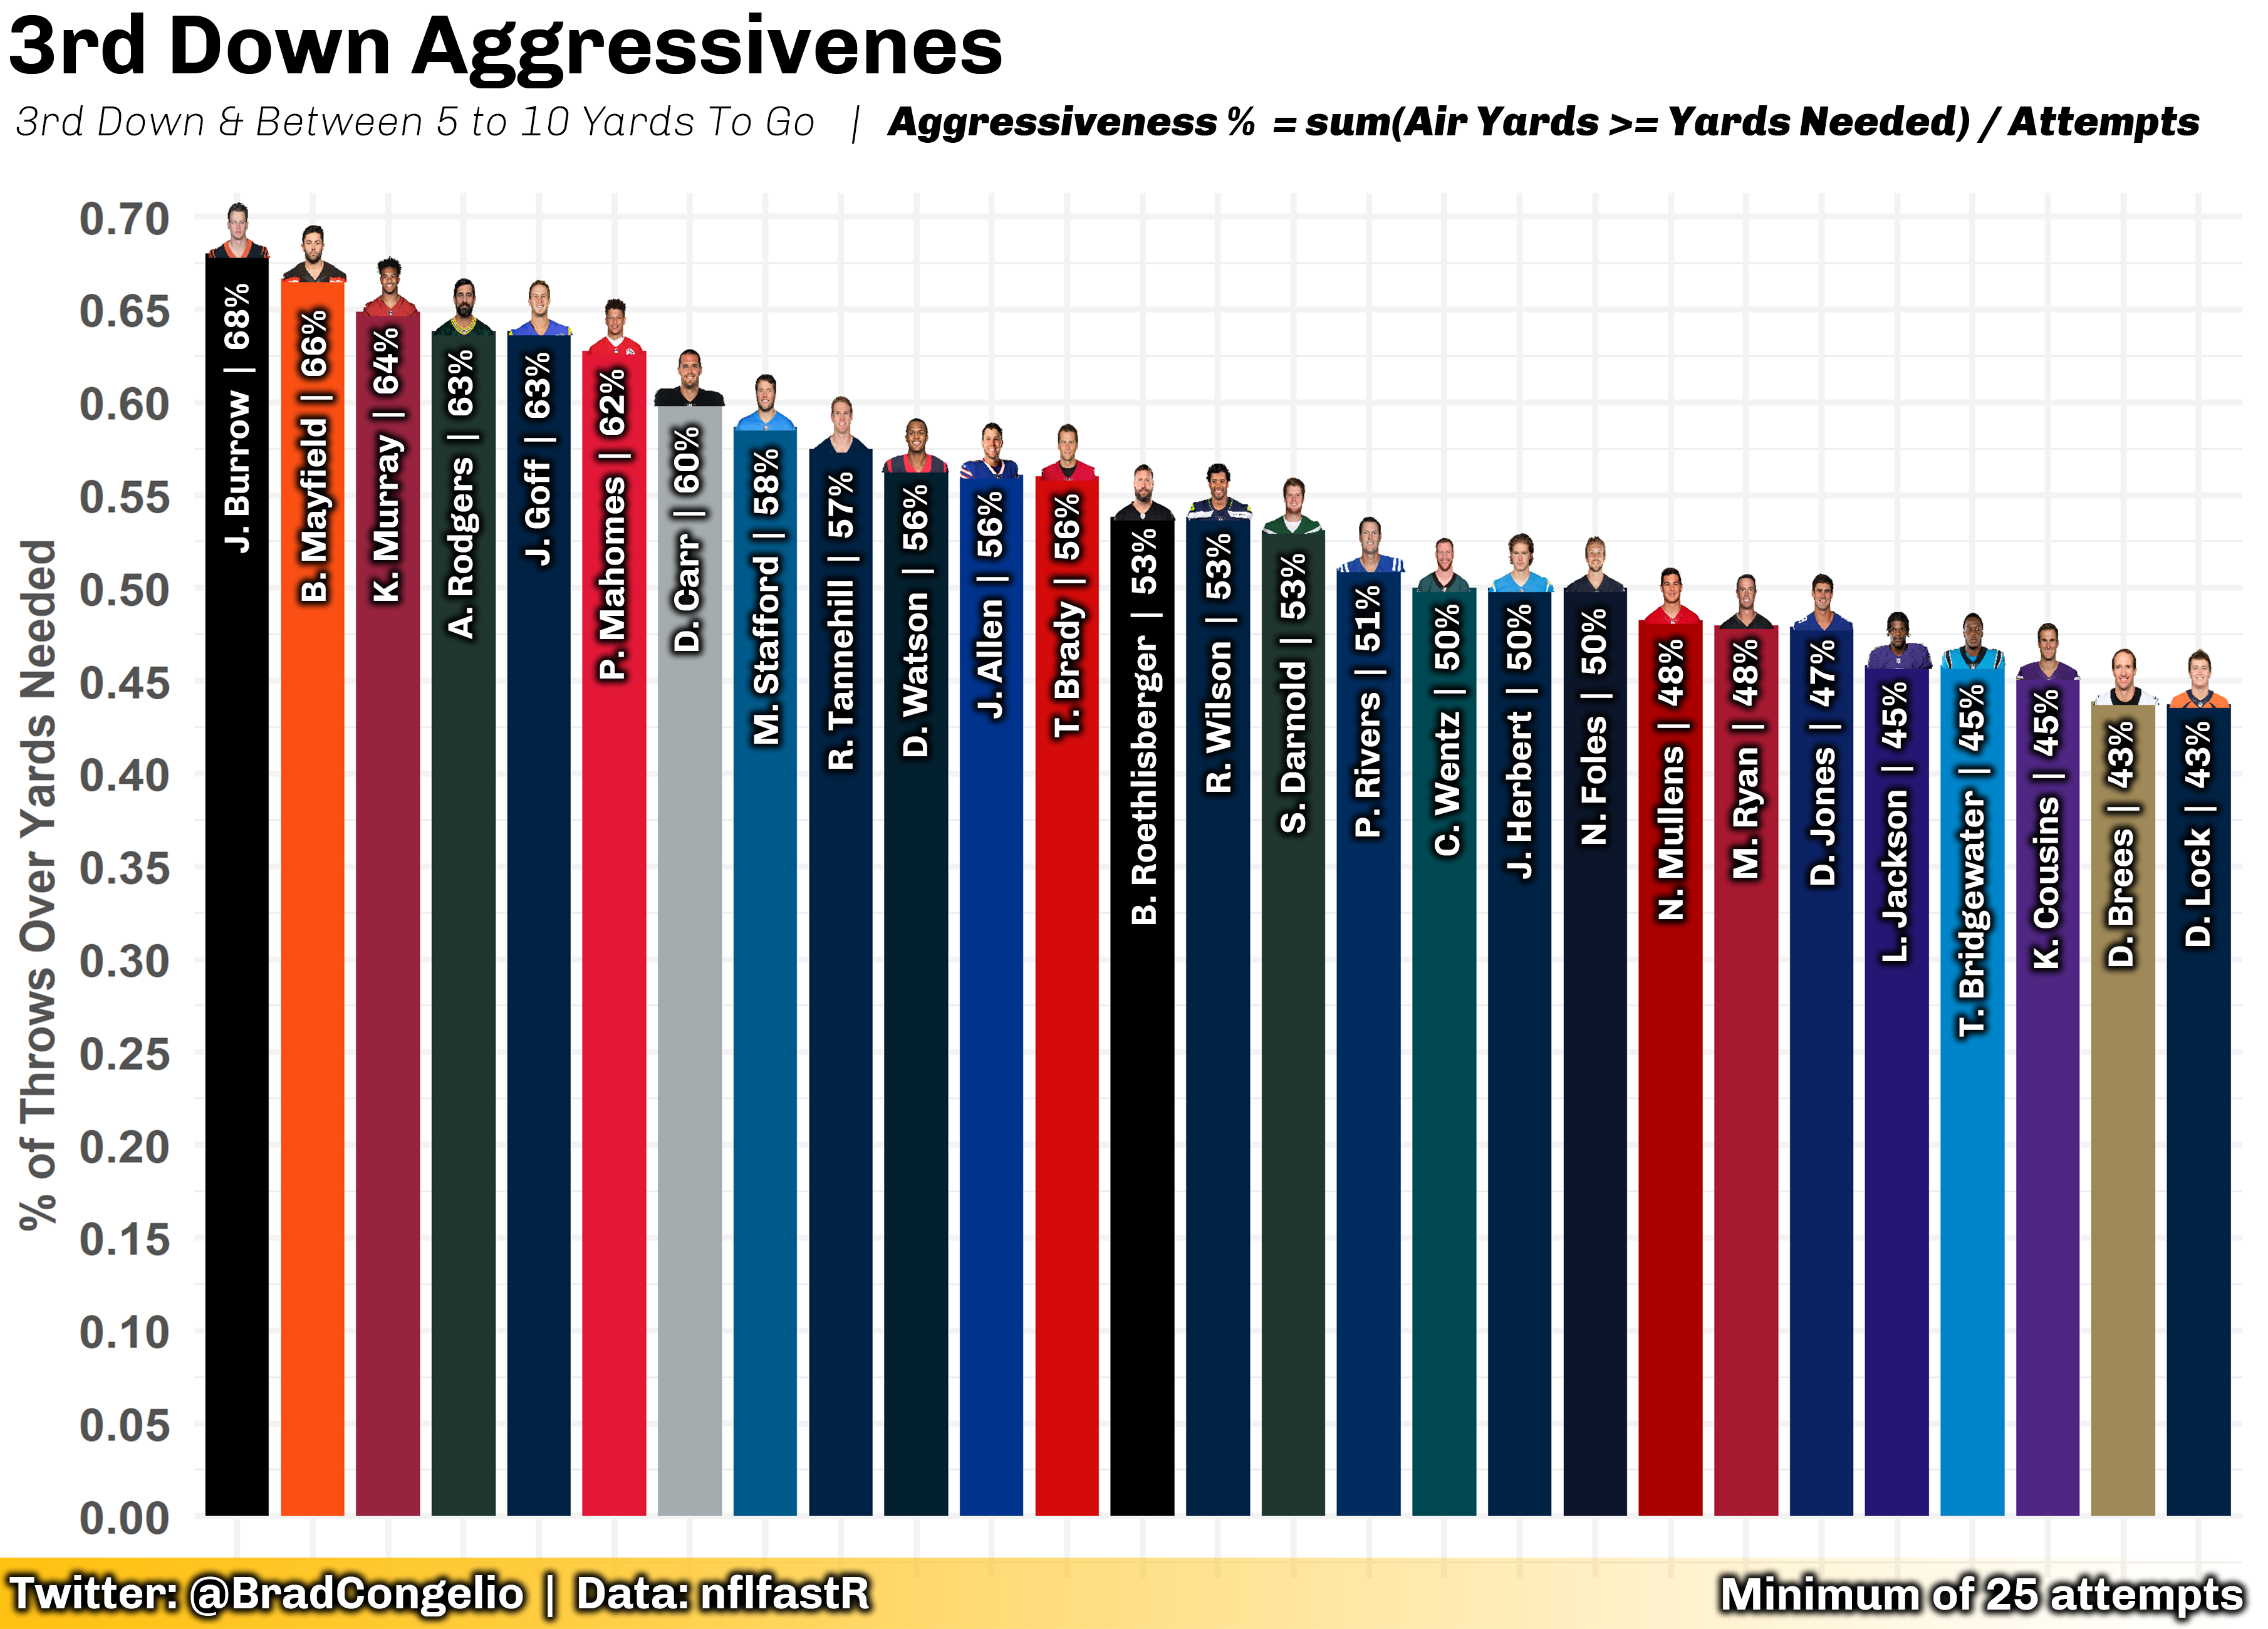
\includegraphics[width=1\textwidth,height=\textheight]{./images/finished-aggressiveness.png}

The above plot explores which QBs, from the 2020 season, were most
aggressive on 3rd down with between 5 to 10 yards to go. Since
``aggressiveness'' is not a typical, day-to-day metric discussed by NFL
fans, I included a ``directable'' within the subtitle of the plot that
explained that the plot, first, was examining just 3rd down pass
attempts within a specific yard range. And, second, I made the decision
to include how ``aggressiveness'' was calculated by including the simple
equation within the subtitle as well. Doing so allows even the most
casual of NFL fans to easily understand what the plot is showing - in
this case, that Joe Burrow's 3rd down pass attempts with between 5 to 10
yards to go made it to the line of gain, or more, on 68\% of his
attempts. On the other hand, Drew Lock and Drew Brees were the least
aggressive QBs in the line based on the same metric.

As another example, below is what I deemed my ``Uncle Rico Metric''
(because who does not like a good Napoleon Dynamite reference?):

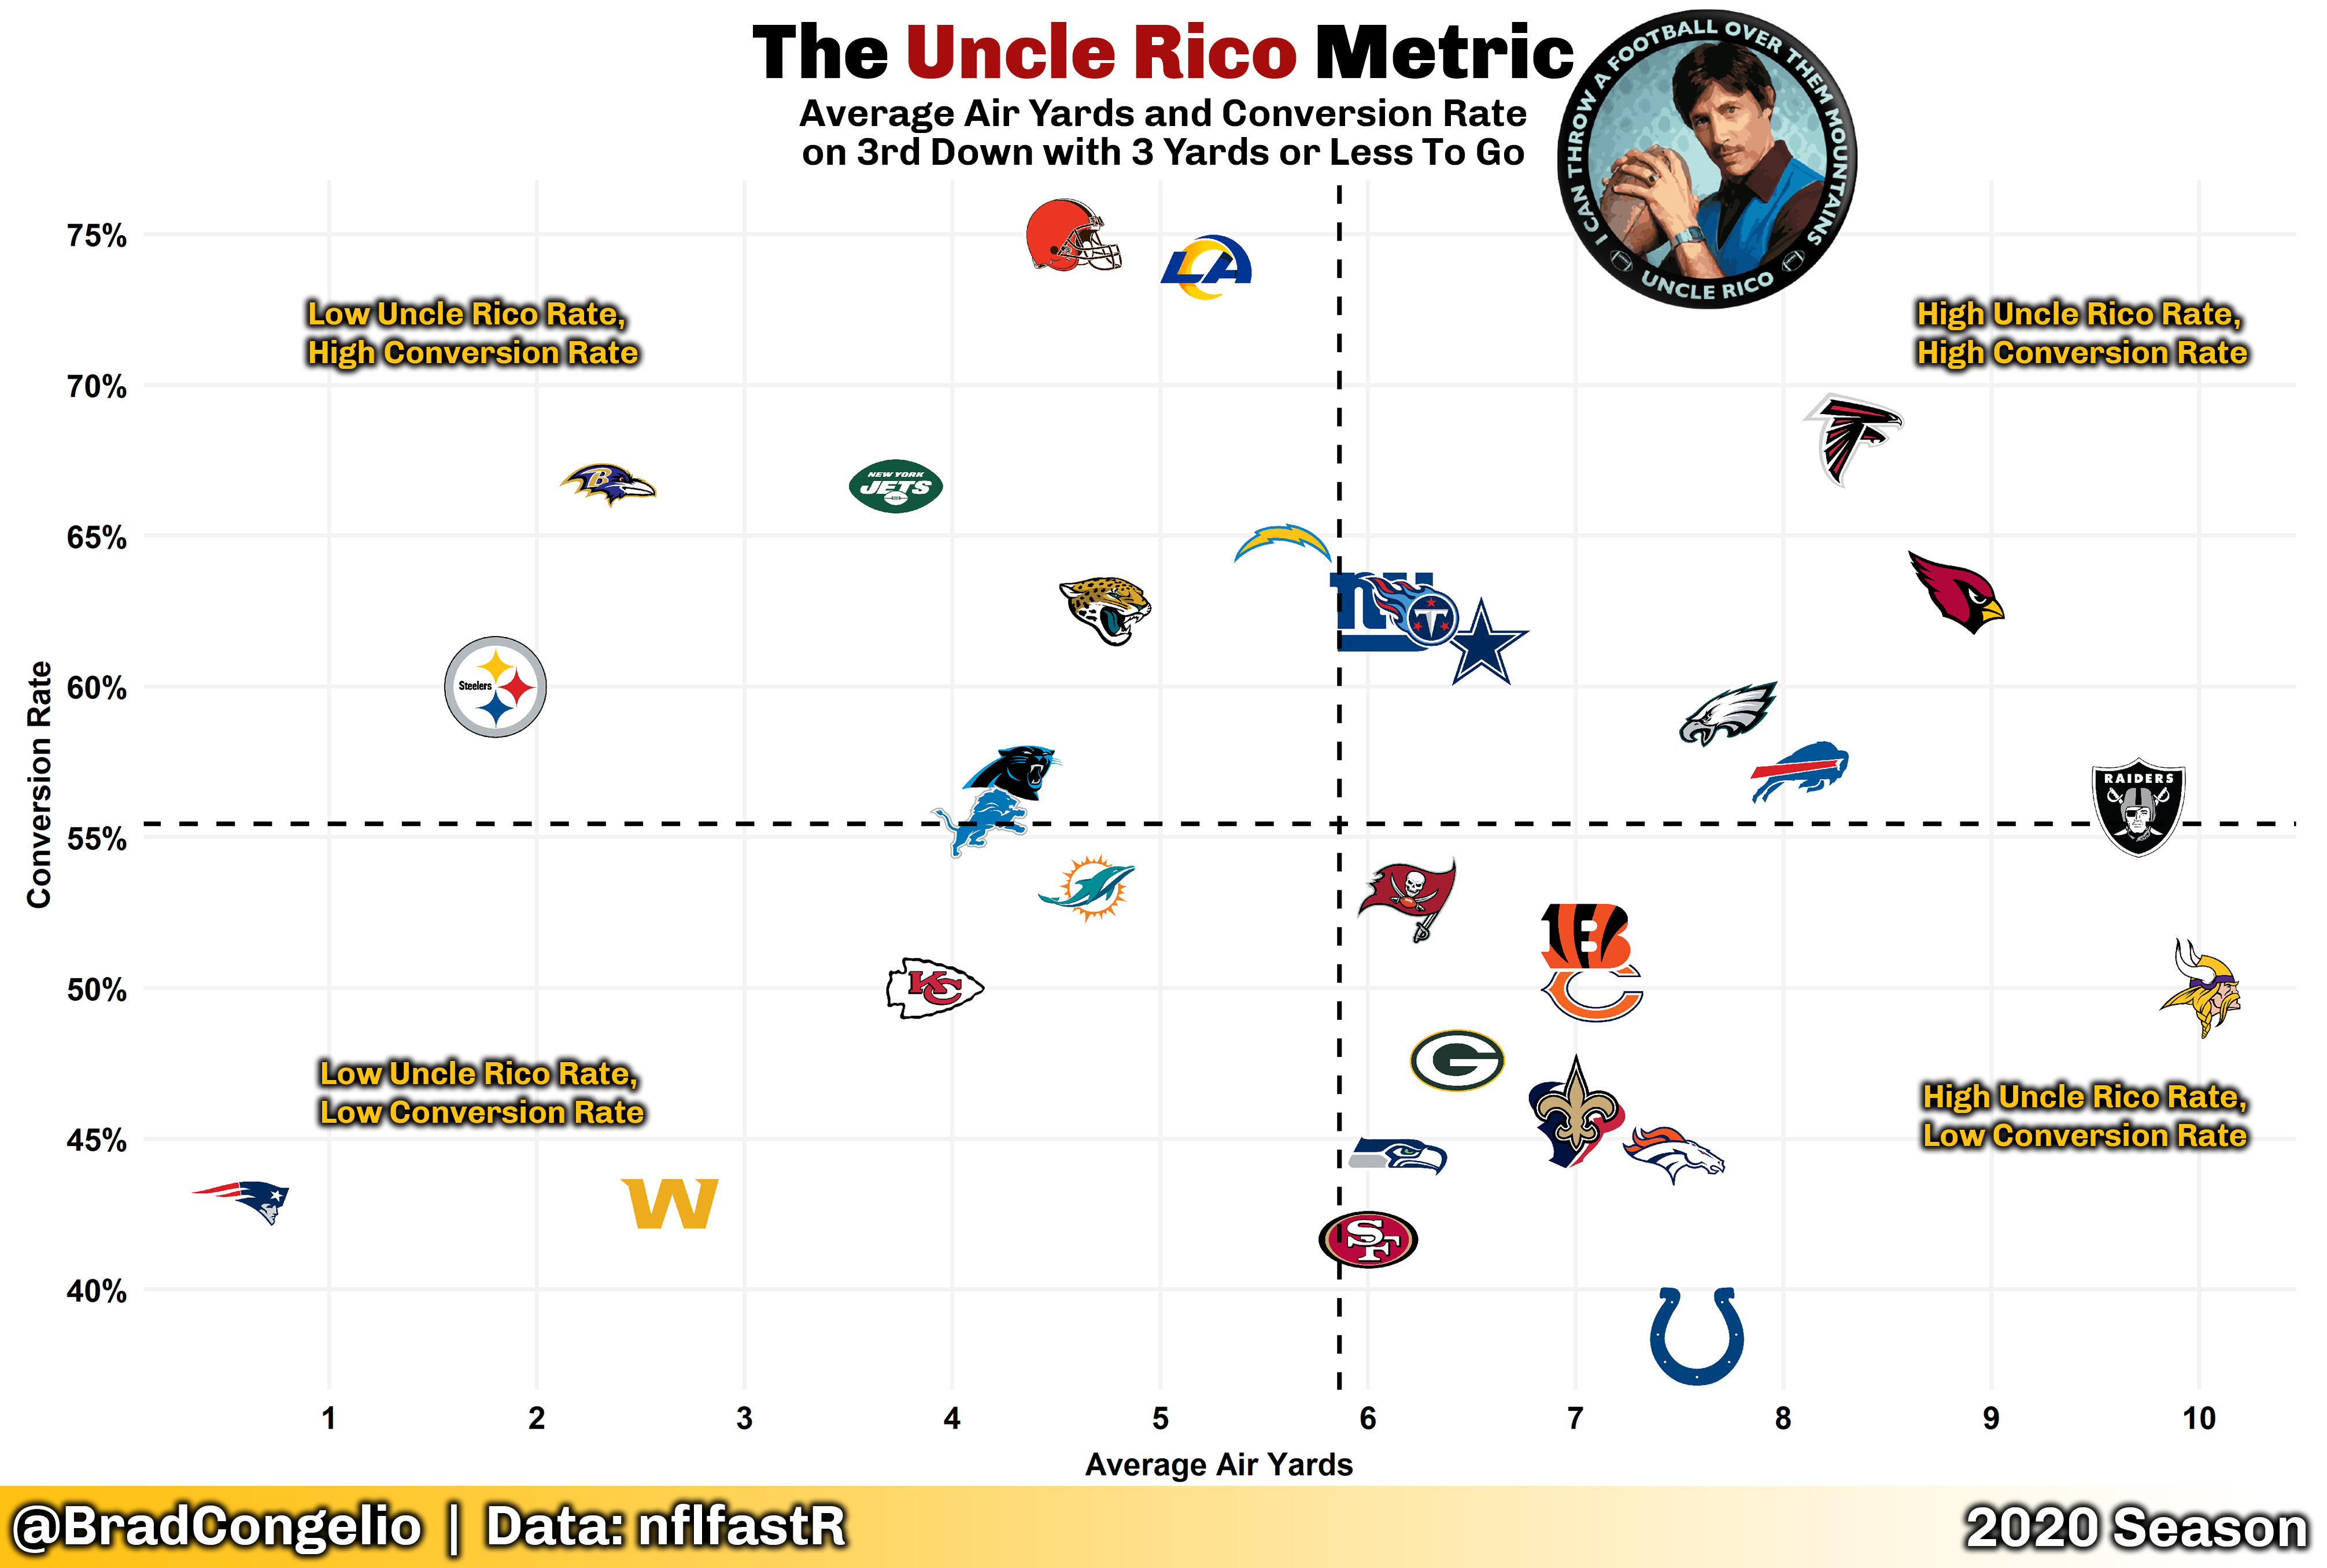
\includegraphics[width=1\textwidth,height=\textheight]{./images/unclerico.png}

\hypertarget{setting-up-for-data-viz}{%
\section{Setting Up for Data Viz}\label{setting-up-for-data-viz}}

While most of your journey through NFL analytics in this book required
you to use the \texttt{tidyverse} and a handful of other packages, the
process of creating compelling and meaningful data visualizations will
require you to utilize multitudes of other packages. Of course, the most
important is \texttt{ggplot2} which is already installed via the
\texttt{tidyverse}. However, in order to recreate the visualizations
included in this chapter, it is required that you install other R
packages. To install the necessary packages, you can run the following
code in RStudio:

\hypertarget{selecting-the-correct-type-of-plot}{%
\section{Selecting The Correct Type of
Plot}\label{selecting-the-correct-type-of-plot}}

\bookmarksetup{startatroot}

\hypertarget{references}{%
\chapter*{References}\label{references}}
\addcontentsline{toc}{chapter}{References}

\hypertarget{refs}{}
\begin{CSLReferences}{1}{0}
\leavevmode\vadjust pre{\hypertarget{ref-awbrey2020}{}}%
Awbrey, Jake. 2020. {``The Future of NFL Analytics.''}
\url{https://www.samford.edu/sports-analytics/fans/2020/The-Future-of-NFL-Data-Analytics}.

\leavevmode\vadjust pre{\hypertarget{ref-bechtold2021}{}}%
Bechtold, Taylor. 2021. {``How the Analytics Movement Has Changed the
NFL and Where It Has Fallen Short.''}
\url{https://theanalyst.com/na/2021/04/evolution-of-the-analytics-movement-in-the-nfl/}.

\leavevmode\vadjust pre{\hypertarget{ref-bigdatabowl-ws}{}}%
{``Big Data Bowl: The Annual Analytics Contest Explores Statistical
Innovations in Football.''} n.d.
\url{https://operations.nfl.com/gameday/analytics/big-data-bowl/}.

\leavevmode\vadjust pre{\hypertarget{ref-bushnell2021}{}}%
Bushnell, Henry. 2021. {``NFL Teams Are Taking 4th-down Risks More Than
Ever - but Still Not Often Enough.''}
\url{https://sports.yahoo.com/nfl-teams-are-taking-4th-down-risks-more-than-ever-but-still-not-often-enough-163650973.html}.

\leavevmode\vadjust pre{\hypertarget{ref-carl2022}{}}%
Carl, Sebastian. 2022. {``nflplotR.''}
\url{https://nflplotr.nflverse.com/}.

\leavevmode\vadjust pre{\hypertarget{ref-fortier2020}{}}%
Fortier, Sam. 2020. {``The NFL's Analytics Movement Has Finally Reached
the Sport's Mainstream.''}
\url{https://www.washingtonpost.com/sports/2020/01/16/nfls-analytics-movement-has-finally-reached-sports-mainstream/}.

\leavevmode\vadjust pre{\hypertarget{ref-heifetz2019}{}}%
Heifetz, Danney. 2019. {``We Salute You, Founding Father of the NFL's
Analytics Movement.''}
\url{https://www.theringer.com/nfl-preview/2019/8/15/20806241/nfl-analytics-pro-football-focus}.

\leavevmode\vadjust pre{\hypertarget{ref-kozora2015}{}}%
Kozora, Alex. 2015. {``Tomlin Prefers "Feel over Analytics".''}
\url{http://steelersdepot.com/2015/09/tomlin-prefers-feel-over-analytics/}.

\leavevmode\vadjust pre{\hypertarget{ref-rosenthal2018}{}}%
Rosenthal, Gregg. 2018. {``Super Bowl LII: How the 2017 Philadelphia
Eagles Were Built.''}
\url{https://www.nfl.com/news/super-bowl-lii-how-the-2017-philadelphia-eagles-were-built-0ap3000000912753}.

\leavevmode\vadjust pre{\hypertarget{ref-silge}{}}%
Silge, Julia. n.d. {``Tidymodels.''} \url{https://tidymodels.org}.

\leavevmode\vadjust pre{\hypertarget{ref-stikeleather2013}{}}%
Stikeleather, Jim. 2013. {``The Three Elements of Successful Data
Visualizations.''}
\url{https://hbr.org/2013/04/the-three-elements-of-successf}.

\end{CSLReferences}

\appendix
\addcontentsline{toc}{part}{Appendices}

\hypertarget{sec-appendix-starting}{%
\chapter{NFL Analytics Reference Guide}\label{sec-appendix-starting}}

This is a work in progress. Reviewers given access to the earliest
version of this book suggest a ``Football 101'' section to bring people
up to speed on analytics and definitions \emph{of} those analytics. This
is going to serve as that reference point, and also include a ``quick
reference guide'' on how to find/calculate the metrics within the
\texttt{nflverse}. Before are just a couple examples of how I see this
section being displayed.

\hypertarget{air-yards}{%
\section{Air Yards}\label{air-yards}}

Air yards is the measure that the ball travels through the air, from the
line of scrimmage, to the exact point where the wide receivers catches,
or does not catch, the football. It does not take into consideration the
amount of yardage gained after the catch by the wide receiver (which
would be \emph{yards after catch}).

For an example, please see the below illustration. In it, the line of
scrimmag is at the 20-yardline. The QB completes a pass that is caught
at midfield (the 50-yardline). After catching the football, the wide
receiver is able to advance the ball down to the opposing 30-yardline
before getting tackled. First and foremost, the quarterback is credited
with a total of 50 passing yards on the play, while the wide receiver is
credited with the same.

However, because air yards is a better metric to explore a QB's
\emph{true} impact on a play, he is credited with 30 air yards while the
wide receiver is credited with 20 yards after catch.

In the end, quarterbacks with higher air yards per attempt are generally
assumed to be throwing the ball deeper downfield than QBs with lower air
yards per attempt.

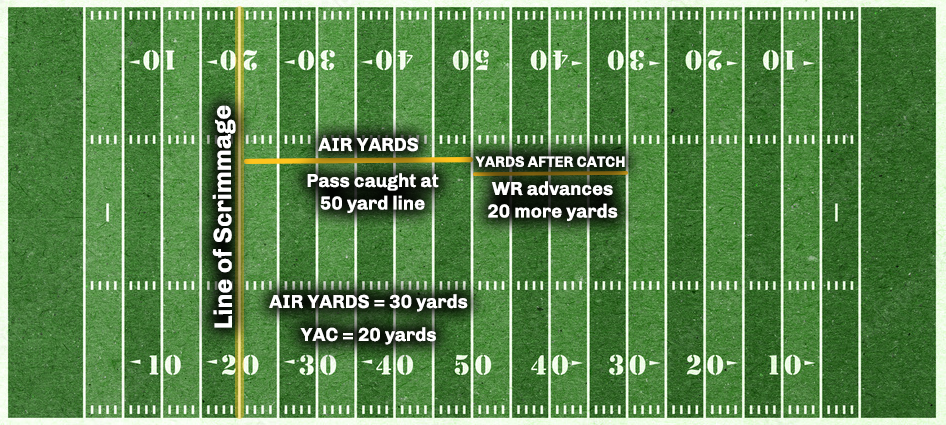
\includegraphics[width=3.15in,height=\textheight]{./images/airyards_101.png}

There are multiple ways to collect data pertaining to air yards.
However, the most straightforward way is to use
\texttt{load\_player\_stats}:

\begin{Shaded}
\begin{Highlighting}[]
\NormalTok{data }\OtherTok{\textless{}{-}}\NormalTok{ nflreadr}\SpecialCharTok{::}\FunctionTok{load\_player\_stats}\NormalTok{(}\DecValTok{2021}\NormalTok{)}

\NormalTok{air.yards }\OtherTok{\textless{}{-}}\NormalTok{ data }\SpecialCharTok{\%\textgreater{}\%}
  \FunctionTok{filter}\NormalTok{(season\_type }\SpecialCharTok{==} \StringTok{"REG"}\NormalTok{) }\SpecialCharTok{\%\textgreater{}\%}
  \FunctionTok{group\_by}\NormalTok{(player\_id) }\SpecialCharTok{\%\textgreater{}\%}
  \FunctionTok{summarize}\NormalTok{(}
    \AttributeTok{attempts =} \FunctionTok{sum}\NormalTok{(attempts),}
    \AttributeTok{name =} \FunctionTok{first}\NormalTok{(player\_name),}
    \AttributeTok{air.yards =} \FunctionTok{sum}\NormalTok{(passing\_air\_yards),}
    \AttributeTok{avg.ay =} \FunctionTok{mean}\NormalTok{(passing\_air\_yards)) }\SpecialCharTok{\%\textgreater{}\%}
  \FunctionTok{filter}\NormalTok{(attempts }\SpecialCharTok{\textgreater{}=} \DecValTok{100}\NormalTok{) }\SpecialCharTok{\%\textgreater{}\%}
  \FunctionTok{select}\NormalTok{(name, air.yards, avg.ay) }\SpecialCharTok{\%\textgreater{}\%}
  \FunctionTok{arrange}\NormalTok{(}\SpecialCharTok{{-}}\NormalTok{air.yards)}

\FunctionTok{tibble}\NormalTok{(air.yards)}
\end{Highlighting}
\end{Shaded}

\begin{verbatim}
# A tibble: 42 x 3
   name       air.yards avg.ay
   <chr>          <dbl>  <dbl>
 1 T.Brady         5821   342.
 2 J.Allen         5295   311.
 3 M.Stafford      5094   300.
 4 D.Carr          5084   299.
 5 J.Herbert       5069   298.
 6 P.Mahomes       4825   284.
 7 T.Lawrence      4732   278.
 8 D.Prescott      4612   288.
 9 K.Cousins       4575   286.
10 J.Burrow        4225   264.
# ... with 32 more rows
\end{verbatim}

In the above example, we can see that Tom Brady led the NFL during the
2021 regular season with a comined total of 5,821 air yards which works
out to an average of 342 air yards per game.

\hypertarget{average-depth-of-target}{%
\section{Average Depth of Target}\label{average-depth-of-target}}

As mentioned above, a QB's air yards per attempt can highlight whether
or not he is attempting to push the ball deeper down field than his
counterparts. The official name of this is \textbf{Average Depth of
Target} (or ADOT). We can easily generate this statistic using the
\texttt{load\_player\_stats} function within \texttt{nflreader}:

\begin{Shaded}
\begin{Highlighting}[]
\NormalTok{data }\OtherTok{\textless{}{-}}\NormalTok{ nflreadr}\SpecialCharTok{::}\FunctionTok{load\_player\_stats}\NormalTok{(}\DecValTok{2021}\NormalTok{)}

\NormalTok{adot }\OtherTok{\textless{}{-}}\NormalTok{ data }\SpecialCharTok{\%\textgreater{}\%}
  \FunctionTok{filter}\NormalTok{(season\_type }\SpecialCharTok{==} \StringTok{"REG"}\NormalTok{) }\SpecialCharTok{\%\textgreater{}\%}
  \FunctionTok{group\_by}\NormalTok{(player\_id) }\SpecialCharTok{\%\textgreater{}\%}
  \FunctionTok{summarize}\NormalTok{(}
    \AttributeTok{name =} \FunctionTok{first}\NormalTok{(player\_name),}
    \AttributeTok{attempts =} \FunctionTok{sum}\NormalTok{(attempts),}
    \AttributeTok{air.yards =} \FunctionTok{sum}\NormalTok{(passing\_air\_yards),}
    \AttributeTok{adot =}\NormalTok{ air.yards }\SpecialCharTok{/}\NormalTok{ attempts) }\SpecialCharTok{\%\textgreater{}\%}
  \FunctionTok{filter}\NormalTok{(attempts }\SpecialCharTok{\textgreater{}=} \DecValTok{100}\NormalTok{) }\SpecialCharTok{\%\textgreater{}\%}
  \FunctionTok{arrange}\NormalTok{(}\SpecialCharTok{{-}}\NormalTok{adot)}

\FunctionTok{tibble}\NormalTok{(adot)}
\end{Highlighting}
\end{Shaded}

\begin{verbatim}
# A tibble: 42 x 5
   player_id  name       attempts air.yards  adot
   <chr>      <chr>         <int>     <dbl> <dbl>
 1 00-0035704 D.Lock          111      1117 10.1 
 2 00-0029263 R.Wilson        400      3955  9.89
 3 00-0036945 J.Fields        270      2636  9.76
 4 00-0034796 L.Jackson       382      3531  9.24
 5 00-0036389 J.Hurts         432      3882  8.99
 6 00-0034855 B.Mayfield      418      3651  8.73
 7 00-0026498 M.Stafford      601      5094  8.48
 8 00-0031503 J.Winston       161      1340  8.32
 9 00-0034857 J.Allen         646      5295  8.20
10 00-0029604 K.Cousins       561      4575  8.16
# ... with 32 more rows
\end{verbatim}

As seen in the results, if we ignore Drew Lock's 10.1 ADOT on just 111
attempts during the 2021 regular season, Russell Wilson attempted to
push the ball, on average, furtherst downfield among QBs with atleast
100 attempts.

\hypertarget{sec-appendix-reading}{%
\chapter{Further Reading Suggestions}\label{sec-appendix-reading}}

This book is, of course, not comprehensive when it comes to highlighting
the R programming language. Because of this, the list below are
suggested readings that will increase your knowledge/skill of R.

\hypertarget{introduction-to-r-programming-books}{%
\section{Introduction to R Programming
Books}\label{introduction-to-r-programming-books}}

\begin{enumerate}
\def\labelenumi{\arabic{enumi}.}
\item
  \href{https://amzn.to/3ovLXUB}{R for Data Science: Import, Tidy,
  Transform, Visualize, and Model Data}
\item
  \href{https://amzn.to/3PYUVWf}{Hands-On Programming with R: Write Your
  Own Functions and Simulations}
\item
  \href{https://amzn.to/3J8lWEv}{The Book of R: A First Course in
  Programming and Statistics}
\item
  \href{https://amzn.to/3zcjYhA}{Learning R: A Step-by-Step Function
  Guide to Data Analysis}
\item
  \href{https://amzn.to/3OBMjn2}{The Art of R Programming: A Tour of
  Statistical Software Design}
\item
  \href{https://amzn.to/3zbBT8f}{Advanced R (Second Edition)}
\end{enumerate}

\hypertarget{data-visualization-in-r-and-visualization-guides}{%
\section{Data Visualization in R and Visualization
Guides}\label{data-visualization-in-r-and-visualization-guides}}

\begin{enumerate}
\def\labelenumi{\arabic{enumi}.}
\item
  \href{https://amzn.to/3oulxTa}{R Graphics Cookbook: Practicl Recipes
  for Visualizing Data}
\item
  \href{https://amzn.to/3PAOB7y}{Storytelling with Data: A Data
  Visualization Guides for Business Professionals}
\item
  \href{https://amzn.to/3PE3QfP}{Better Data Visualizations: A Guide for
  Scholars, Researchers, and Wonks}
\end{enumerate}

\hypertarget{sport-analytics-guidesbooks}{%
\section{Sport Analytics
Guides/Books}\label{sport-analytics-guidesbooks}}

\begin{enumerate}
\def\labelenumi{\arabic{enumi}.}
\item
  \href{https://amzn.to/3PE2LEK}{The Midrange Theory: Basketball's
  Evolution in the Age of Analytics}
\item
  \href{https://amzn.to/3vgIyNl}{Analyzing Baseball Data with R (2nd
  edition)}
\item
  \href{https://amzn.to/3zwXcCA}{A Fan's Guide to Baseball Analytics:
  Why WAR, WHIP, wOBA, and other Advanced Sabermetrics Are Essential to
  Understanding Modern Baseball}
\item
  \href{https://amzn.to/3vgR3rM}{The Book: Playing the Percentages in
  Baseball}
\item
  \href{https://amzn.to/3oy66t4}{The Hidden Game of Baseball: A
  Revolutionary Approach to Baseball and Its Statistics}
\item
  \href{https://amzn.to/3PZt7kf}{The Hidden Game of Football: A
  Revealing and Lively Look at the Pro Game, With New Stats,
  Revolutionary Strategies, and Keys to Picking the Winners}
\item
  \href{https://amzn.to/3zwXysU}{Mathletics: How Gamblers, Managers, and
  Fans Use Mathematics in Sports}
\item
  \href{https://amzn.to/3Bnd23U}{Basketball Data Science: With
  Applications in R}
\item
  \href{https://amzn.to/3PE4bPA}{Data Analytics in Football (Soccer):
  Positional Data Collection, Modelling, and Analysis}
\end{enumerate}



\end{document}
